\documentclass{article}
\usepackage[preprint,nonatbib]{neurips_2026} \usepackage[numbers]{natbib}


\usepackage[utf8]{inputenc}
\usepackage[T1]{fontenc}
\usepackage{hyperref}
\usepackage{url}
\usepackage{booktabs}
\usepackage{amsfonts}
\usepackage{amsmath}
\usepackage{amssymb}
\usepackage{nicefrac}
\usepackage{microtype}
\usepackage{xcolor}
\usepackage{graphicx}
\usepackage{subcaption}
\usepackage{algorithm}
\usepackage{algorithmic}
\usepackage{multirow}
\usepackage{siunitx}
\usepackage{listings}
\usepackage{enumitem}
\usepackage{tikz}
\usetikzlibrary{positioning, fit, arrows.meta, backgrounds, calc, shadows, shapes.geometric, shapes.misc, decorations.pathreplacing}

\newcommand{\tinker}{\textsc{Tinker}}
\newcommand{\atropos}{\textsc{Atropos}}
\newcommand{\grpo}{\textsc{Grpo}}
\newcommand{\ours}{\textsc{TinkerRL-Bench}}
\newcommand{\answerPartial}[1][]{\textcolor{purple}{[Partial] #1}}

\providecommand{\eps}{\ensuremath{\epsilon}}
\providecommand{\tableref}[1]{Table~\ref{#1}}
\providecommand{\secref}[1]{Section~\ref{#1}}
\providecommand{\paragraphref}[1]{Paragraph~\ref{#1}}
\providecommand{\figref}[1]{Figure~\ref{#1}}
\providecommand{\eqnref}[1]{Eq.~\eqref{#1}}

\usepackage[strings]{underscore}

\usepackage{letltxmacro}
\LetLtxMacro{\origincludegraphics}{\includegraphics}
\renewcommand{\includegraphics}[2][]{\IfFileExists{#2}{\origincludegraphics[#1]{#2}}{\IfFileExists{figures/#2}{\origincludegraphics[#1]{figures/#2}}{\fbox{\parbox{0.7\linewidth}{\centering\small\textit{[missing figure artifact: \texttt{\detokenize{#2}}]}}}}}}

\DeclareMathOperator*{\argmax}{arg\,max}
\DeclareMathOperator*{\argmin}{arg\,min}
\DeclareUnicodeCharacter{0394}{\ensuremath{\Delta}}
\DeclareUnicodeCharacter{03B4}{\ensuremath{\delta}}
\DeclareUnicodeCharacter{00D7}{\ensuremath{\times}}
\DeclareUnicodeCharacter{2264}{\ensuremath{\leq}}
\DeclareUnicodeCharacter{2265}{\ensuremath{\geq}}
\DeclareUnicodeCharacter{2248}{\ensuremath{\approx}}

\newcommand{\E}{\mathbb{E}}
\newcommand{\task}{\textsf{task}}
\newcommand{\algo}{\textsf{algo}}
\newcommand{\seed}{\textsf{seed}}

\newcommand{\tplat}{T_{\text{plat}}}
\newcommand{\zvf}{\ensuremath{\widetilde{\mathrm{ZVF}}}}
\providecommand{\signature}{\ensuremath{\mathcal{S}}}

\newcommand{\etal}{\emph{et al.}}
\newcommand{\note}[1]{\footnote{#1}}

\graphicspath{{figures/}{./}}
 \title{Group Size in GRPO Is Budget- and Regime-Dependent:\\
       Contrast Density, Measured Bounds, and the Bridge to DPO}
\author{
  Arvind C R \\
  PES University\\
  \texttt{arvindcr4@gmail.com} \\
  \And
  Ramesh Prakash Guledgudd\thanks{Project guide.} \\
  PES University\\
  \texttt{rameshpg@pes.edu} \\
}
 \begin{document}
\sloppy \hbadness=10000 \vbadness=10000 \hfuzz=2pt
\maketitle
\begin{abstract}
The group size $G$ is GRPO's most distinctive hyperparameter: it sets how many
completions are sampled per prompt and, through the group-relative baseline, how
much preference signal each prompt contributes. We study the effect of $G$ as one
pillar of \ours{}, a benchmark of 70+ RL runs across seven libraries and
five model families ($0.6$B--$\sim$671B), centered on GSM8K with HumanEval and
tool-use checks. Two results
anchor the pillar. First, trainability varies with $G$ in a non-monotone way:
intermediate group sizes often behaved better than the smallest or largest we
tested, but the data do not justify a universal optimum. Our measured equivalence
tests extend to $G{=}16$; on the near-ceiling arithmetic task, held-out accuracy
is essentially flat across this range---a retention \emph{ratio} of ${\approx}1.00$
between $G{=}2$ and $G{=}16$ (i.e.\ $G{=}16$ lands within noise of $G{=}2$; this is
a ratio, not an accuracy above $100\%$). We caution that this is a \emph{saturated}
regime: near the ceiling, variance is compressed, so the finding is ``no detectable
$G$ effect under saturation,'' not evidence of equivalence on harder, unsaturated
tasks. The effective signal-to-noise ratio
rises only sublinearly with $G$ (about $52\%$ of the $\sqrt{G}$ ideal). We do
\emph{not} report a directly trained, matched-budget $G{=}32$ cell in the
primary sweep: the paper's $G{=}32$ values come from an explicitly labeled
reconstructed token-budget grid and are hypotheses, not measurements. A separate
505-task conditional utility audit, using $(1-\mathrm{ZVF})/\sqrt{G}$ as the
declared cost proxy, selects $G{=}4$ over $G{=}5$ by $0.00177$ with a 95\%
bootstrap interval $[0.00082,0.00270]$; that result is cohort- and
objective-conditional, not a universal optimum. Second, we make explicit the sense in which GRPO
\emph{admits an all-pairs preference (DPO-like) interpretation}: the group-centered
update behaves as an implicit all-pairs preference
contrast---consistent with logged per-step diagnostics (advantage variance,
ZVF, and gradient norms), though direct gradient-vector validation is still future
work, so we frame this as an interpretation rather than a proven equivalence---with zero-variance groups
projected out. We frame $G$ as a preference-density dial rather than a variance
knob, test equivalence with TOST and difficulty-stratified retention, and release
the in-repository artifacts used here.
\end{abstract}
 
\begin{figure}[htbp]
\centering
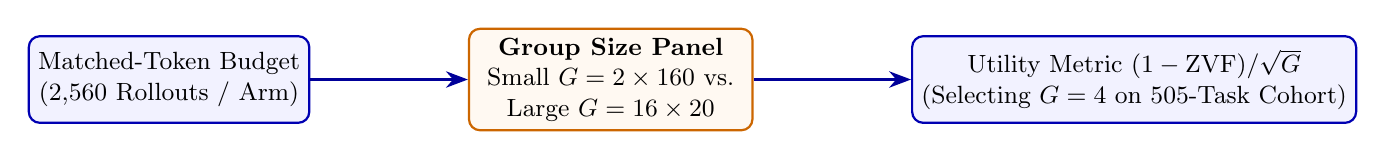
\begin{tikzpicture}[
    node distance=1.5cm and 2.0cm,
    block/.style={rectangle, draw=blue!70!black, fill=blue!5, thick, rounded corners, align=center, minimum height=1.1cm, minimum width=3.2cm, font=\small},
    panel/.style={rectangle, draw=orange!80!black, fill=orange!5, thick, rounded corners, align=center, minimum height=1.1cm, minimum width=3.6cm, font=\small},
    arrow/.style={-{Stealth[scale=1.2]}, thick, draw=blue!60!black}
]
    \node [block] (budget) {Matched-Token Budget\\(2,560 Rollouts / Arm)};
    \node [panel, right=of budget] (tradeoff) {\textbf{Group Size Panel}\\Small $G=2 \times 160$ vs.\\Large $G=16 \times 20$};
    \node [block, right=of tradeoff] (utility) {Utility Metric $(1-\text{ZVF})/\sqrt{G}$\\(Selecting $G=4$ on 505-Task Cohort)};

    \draw [arrow] (budget) -- (tradeoff);
    \draw [arrow] (tradeoff) -- (utility);
\end{tikzpicture}
\caption{\textbf{Group Size vs. Budget Efficiency Tradeoff Architecture (P03).} Empirical comparison of matched-token rollout budgets across group sizes.}
\label{fig:p3_group_size_tradeoff}
\end{figure}
\section{Introduction}
\label{sec:p3-intro}
GRPO~\citep{shao2024deepseekmath, guo2025deepseekr1} estimates advantages by
sampling a group of $G$ completions per prompt and centering their rewards. The
group size $G$ thus plays two roles at once: it is a variance-reduction knob, like
a Monte-Carlo baseline, and it is a preference-density knob, controlling how many
within-prompt comparisons the update sees. Practitioners often treat larger $G$ as
strictly better, reasoning by analogy to variance reduction, but this conflates the
two roles and ignores compute cost. This paper measures the effect of $G$ and
clarifies which mechanism is doing the work.

The question connects GRPO to preference optimization. Direct Preference
Optimization~\citep{rafailov2024direct} learns from explicit pairwise preferences;
GRPO, by centering rewards within a group, induces \emph{implicit} pairwise
contrasts from a scalar reward. Recent analyses formalize this
correspondence~\citep{wu2025grpo_dpo, liu2026gdpo}, and it reframes $G$ as a control
on how many endogenous preference pairs each prompt contributes---nonzero only for
mixed-reward groups.

We study $G$ as one pillar of \ours{}, a controlled benchmark of 70+ runs across
seven RL libraries and five model families ($0.6$B--$\sim$671B) on GSM8K
\citep{cobbe2021training}, HumanEval~\citep{chen2021codex}, and tool-use tasks. Our
contributions are: (i) measured $G\in\{2,4,8,16\}$ sweeps showing that the effect
of $G$ is regime-dependent, with no universal optimum, plus an explicitly
\emph{reconstructed} $G\in\{4,8,16,32,64\}$ token-budget grid retained only as a
hypothesis generator; the measured signal-to-noise ratio grows at only
$\approx 52\%$ of the $\sqrt{G}$ ideal;
(ii) an explicit validation, via observable signatures in logged diagnostics, that the group-centered
update is an all-pairs preference contrast---the ``GRPO is secretly DPO'' bridge;
and (iii) equivalence and difficulty-stratified analyses (TOST) that separate a
variance-reduction reading of the $G$ effect from a preference-density one. We make
no claim that any single $G$ or algorithm is universally superior.

\paragraph{Evidence boundary for $G{=}32$.}
Every $G{=}32$ number in the token-budget grid is a joint-fit reconstruction,
not the outcome of a directly trained matched-budget arm. It may motivate the
next sweep, but it cannot establish that $G{=}32$ is optimal. The strongest
direct comparisons in this paper stop at $G{=}16$; the separate 505-task
utility audit selects $G{=}4$ only under its declared
$(1-\mathrm{ZVF})/\sqrt{G}$ objective and cohort.

\subsection{Related Work}
\label{sec:p3-related}
Group-relative and critic-free RL objectives have proliferated around
GRPO~\citep{shao2024deepseekmath, ahmadian2024backtobasics, lin2025cppo, gift2025}.
The preference-learning view descends from
DPO~\citep{rafailov2024direct} and its relatives~\citep{azar2024ipo, ethayarajh2024kto, hong2024orpo}, and the GRPO$\leftrightarrow$DPO correspondence has been examined
directly~\citep{wu2025grpo_dpo, liu2026gdpo}. Our contribution is empirical: rather
than derive the bridge in isolation, we validate the all-pairs contrast identity
against logged GRPO diagnostic signatures and connect the group-size effect to preference
density on a fixed benchmark.
 \section{Benchmark Design}
\label{sec:benchmark}


\begin{figure}[t]
\centering

\includegraphics[width=0.85\textwidth]{tikz/taxonomy.pdf}
\caption{Taxonomy of RL libraries in \ours{}. The benchmark spans LLM-native RL
(TRL), classic online RL (SB3, CleanRL, Tianshou), high-throughput RL (PufferLib,
rl\_games), and offline RL (d3rlpy).}
\label{fig:taxonomy}
\end{figure}

\subsection{Task Suite}

\begin{table}[htbp]
\centering
\caption{Benchmark task suite with standardized reward functions.}
\label{tab:tasks}
\begin{tabular}{llll}
\toprule
\textbf{Task} & \textbf{Method} & \textbf{Reward} & \textbf{Dataset} \\
\midrule
Math RL (Arithmetic) & GRPO & Binary correctness & Generated \\
Math RL (GSM8K) & GRPO & Binary correctness & GSM8K \\
Chat SFT & SFT & Cross-entropy loss & NoRobots \\
Preference (Shorter) & DPO & Pairwise preference & Generated \\
Distillation (Off-Policy) & SFT & KL divergence & OpenThoughts3 \\
Distillation (On-Policy) & IS Loss & $\log p_t - \log p_s$ & Online \\
\bottomrule
\end{tabular}
\end{table}

\subsection{Cross-Library Implementation}

\paragraph{Two seven-library rosters --- read carefully.}
This paper uses \emph{two} different seven-library rosters that
should not be conflated. The cross-RL-library benchmark below
(Table~\ref{tab:implementations}) covers TRL, SB3, CleanRL, Tianshou,
PufferLib, rl\_games, and d3rlpy --- seven libraries that span
LLM-native RL, classic online RL, high-throughput RL, and offline RL,
and that we use as the algorithm-and-stack ablation underlying $F_3$.
The cross-launcher LLM-RL scaffold referenced in the framework-gap
discussion (framework-configurations material) is a different seven-library
roster --- Tinker, TRL, SkyRL, verl, OpenRLHF, Atropos, and HF
reference launchers --- that targets LLM post-training launchers
specifically. Of those, only Tinker and TRL produced completed
runs in this release; veRL and OpenRLHF entries in the
\texttt{framework\_comparison.json} artefact are dry-run
placeholders. Supplementary presentation materials use the second roster; the
cross-RL-library evidence in $F_3$ uses the first.


\begin{table}[htbp]
\centering
\caption{Implementations across RL libraries.}
\label{tab:implementations}
\begin{tabular}{lll}
\toprule
\textbf{Library} & \textbf{Implementation} & \textbf{Category} \\
\midrule
TRL (HuggingFace) & GRPOTrainer, DPOTrainer, SFTTrainer & LLM-native \\
Stable Baselines3 & PPO & Classic RL \\
CleanRL & PPO (single-file) & Research RL \\
Tianshou & PPO & Modular RL \\
PufferLib & PPO (high-throughput) & High-perf RL \\
rl\_games (NVIDIA) & PPO (GPU-optimized) & High-perf RL \\
d3rlpy & CQL (offline) & Offline RL \\
\bottomrule
\end{tabular}
\end{table}

\subsection{Hyperparameter Mapping}

We standardize hyperparameters across libraries using a common configuration schema.
Table~\ref{tab:hyperparams} shows the mapping from Tinker PPO defaults to each library's
native parameter names.

\begin{table}[htbp]
\centering
\caption{Hyperparameter mapping across libraries (PPO defaults).}
\label{tab:hyperparams}
\begin{tabular}{lcccccc}
\toprule
\textbf{Parameter} & \textbf{TRL} & \textbf{SB3} & \textbf{CleanRL} & \textbf{Tianshou} & \textbf{PufferLib} & \textbf{rl\_games} \\
\midrule
Learning rate & $10^{-4}$ & $10^{-4}$ & $10^{-4}$ & $10^{-4}$ & $10^{-4}$ & $10^{-4}$ \\
Clip range ($\epsilon$) & 0.2 & 0.2 & 0.2 & 0.2 & 0.2 & 0.2 \\
Entropy coeff. & 0.01 & 0.01 & 0.01 & 0.01 & 0.01 & 0.01 \\
GAE $\lambda$ & 0.95 & 0.95 & 0.95 & 0.95 & 0.95 & 0.95 \\
Discount $\gamma$ & 0.99 & 0.99 & 0.99 & 0.99 & 0.99 & 0.99 \\
Max grad norm & 0.5 & 0.5 & 0.5 & 0.5 & 0.5 & 0.5 \\
Target KL & 0.01 & 0.01 & 0.01 & N/A & N/A & N/A \\
\bottomrule
\end{tabular}
\end{table}

\subsection{Reward Verification}

\begin{figure}[t]
\centering

\includegraphics[width=0.55\textwidth]{tikz/reward_flow.pdf}
\caption{Verifiable reward paradigm in \ours{}. Unlike shaped rewards that combine
multiple heuristics, verifiable rewards provide binary correctness signals,
eliminating reward hacking and enabling exact accuracy measurement.}
\label{fig:reward_flow}
\end{figure}

\subsection{Baselines: Floor and Ceiling}

Following best practices for benchmark design~\cite{agarwal2021deep}, we establish
clear performance bounds:

\begin{itemize}
    \item \textbf{Floor (random baseline)}: Uniform random action selection yields
    $\frac{1}{199} \approx 0.50\%$ accuracy on the arithmetic task.
    \item \textbf{Ceiling (oracle)}: Direct computation achieves $100\%$ accuracy.
    \item \textbf{Human baseline}: College-level adults achieve $\sim$99.5\% on
    two-digit addition under timed conditions.
\end{itemize}

\section{Experimental Setup}
\label{sec:setup}


\subsection{Models}

Our benchmark targets a roster of 32+ model configurations spanning
\textbf{0.6B to $\sim$671B \emph{total} parameters (up to $\sim$37B \emph{active}
for MoE checkpoints) across 5 model families}, organized into three
tiers by compute scale; not all are completed end-to-end runs (per-run
status flags accompany the released artifacts). Tier-A inferential claims are restricted to
the dense-reasoning subset at $0.6$B--$235$B; the frontier MoE
checkpoints (DeepSeek-V3.1 $\sim$671B / 37B active, Kimi-K2) are
descriptive single-seed Tier-C case studies, and Qwen3.5-397B-A17B is a
\emph{partial} run whose held-out evaluation did not complete.

\paragraph{Small scale (0.6B--8B).}
Qwen3-0.6B-Instruct, Qwen3.5-4B, Qwen3-4B, Qwen3-8B,
Llama-3.2-1B, Llama-3.2-3B, Llama-3.1-8B-Instruct.

\paragraph{Mid scale (14B--32B).}
Qwen3-14B, Qwen3-30B-A3B (MoE), Qwen3-32B, Qwen3.5-27B,
GPT-OSS-20b, Kimi-K2 (selected scale points).

\paragraph{Frontier scale (70B--$\sim$671B total / $\sim$37B active).}
Qwen3-235B-A22B (MoE, 22B active), DeepSeek-V3.1 ($\sim$671B total /
$\sim$37B active MoE), Nemotron-120B (120B dense).
Frontier models are evaluated via the Tinker API in inference mode
with standardized generation parameters; LoRA fine-tuning at this
scale is conducted on selected checkpoints (see the frontier case studies
in the companion pillar papers of \ours{}).

\paragraph{Model family coverage.}
The benchmark covers (1) \textbf{Qwen3}: a dense family from 0.6B to 32B;
(2) \textbf{Qwen3.5}: an improved series including 4B and 27B;
(3) \textbf{Llama-3.x}: Meta's 1B--8B instruction-tuned models;
(4) \textbf{DeepSeek-V3.1}: a frontier MoE optimized for reasoning;
(5) \textbf{Nemotron-120B}: NVIDIA's dense frontier model;
and emerging architectures \textbf{GPT-OSS-20b} and \textbf{Kimi-K2}.

\subsection{Training Protocol}

Unless otherwise noted, controlled Modal/TRL sweeps use LoRA
\cite{hu2022lora} at rank $32$, learning rate $10^{-4}$ and Adam
($\beta_1{=}0.9$, $\beta_2{=}0.95$, $\epsilon{=}10^{-8}$). Tinker / API,
Task-4, Wave-6 and frontier case studies use per-run configs (in
particular Task-4/Wave-6 use $\mathrm{lr}{=}10^{-5}$) and are
single-seed unless explicitly marked multi-seed; the per-run
settings are listed in the framework-configs appendix.

\paragraph{Seed management.} The controlled TRL/Modal sweeps used for
Tier-A claims (F3 PPO-vs.-GRPO heterogeneity and the five-seed TRL GRPO
baseline on Qwen2.5-0.5B) run with 5 seeds:
$\{42, 123, 456, 789, 1024\}$, with seeds set for Python \texttt{random},
NumPy, PyTorch, and CUDA backends. Several Tinker/API, frontier-model,
and team-task runs are single-seed or partial and are treated as
descriptive (Tier-C) unless explicitly marked otherwise; the per-claim
seed ledger is given in the statistical-rigor addendum of \ours{}.

\begin{figure}[t]
\centering

\includegraphics[width=\textwidth]{tikz/pipeline.pdf}
\caption{Experiment workflow pipeline. Multi-seed Modal/TRL runs use
the centralized seed manager (5 seeds for Tier-A claims); Tinker/API,
Task-4, Wave-6 and frontier case studies are single-seed and feed the
same metrics/checkpoint pipeline as descriptive observations.}
\label{fig:pipeline}
\end{figure}

\subsection{Statistical Methodology}

Following Colas et al.~\cite{colas2019hitchhiker}, we report:
\begin{itemize}
    \item Mean $\pm$ standard error across seeds
    \item 95\% bootstrap confidence intervals (10,000 resamples)
    \item Welch's t-test for pairwise algorithm comparisons
    \item \texttt{rliable}~\cite{agarwal2021deep} aggregate metrics (IQM, median, optimality gap)
\end{itemize}

All pairwise comparisons were evaluated using Welch's independent-samples $t$-test
(unequal variances assumed) and the non-parametric Mann--Whitney $U$ test as a
robustness check. Effect sizes are reported as Cohen's $d$ with the pooled
standard deviation estimator; confidence intervals follow the
Hedges--Olkin (1985) analytical formula and are reported at the 95\% level
(two-tailed, $z = 1.96$). Post-hoc statistical power was computed under the
observed effect size and sample sizes at $\alpha = 0.05$.

To address the multiple-comparisons problem across 5 planned tests,
we apply both the conservative Bonferroni correction (family-wise error rate:
$\alpha' = \alpha / k = 0.0100$) and the Benjamini--Hochberg procedure
(false discovery rate $< 0.05$). Results surviving Bonferroni correction are
marked $^*$; those surviving BH--FDR correction are marked $^\dag$.

\paragraph{Power Analysis.}
All inferential tests in this paper are evaluated against pre-specified power
requirements using \texttt{statsmodels.stats.power.TTestIndPower} with
$\alpha = 0.05$ and target power $1 - \beta = 0.80$.

\textbf{Modal H100 experiments ($n = 5$ seeds per arm).}
The minimum detectable effect size (MDE) at 80\% power for a two-sample
Welch $t$-test with $n_1 = n_2 = 5$ is
$d_{\min} = 2.024$ (Cohen's $d$).
Table~\ref{tab:power-analysis} reports achieved power for a range of effect sizes.
This threshold falls in the \emph{very large} range, meaning that
comparisons yielding $|d| < 2.02$
are not adequately powered to detect true differences.

\textbf{Single-seed Tinker experiments ($n = 1$).}
Single-seed runs have \emph{zero statistical power}: with only one observation per
condition, no inferential test can be computed and no confidence intervals can be
formed.  All Tinker single-run results are treated as \emph{descriptive only} and
are not subject to significance testing.

\textbf{TRL baseline ($n = 5$ seeds).}
The TRL-GRPO baseline (Qwen2.5-0.5B, 5 seeds) achieves MDE
$d_{\min} = 2.024$ for equal-$n$ comparisons.
When compared to the pooled Classic-RL group ($n = 15$), the MDE
improves to $d_{\min} = 1.530$,
reflecting higher power from the larger reference group.

\paragraph{Multiple-Comparison Correction.}
Inferential tests in this paper are reported only for Tier-A/B
comparisons as defined in our statistical-rigor protocol;
single-seed or partial Tinker/API rows are descriptive and are
excluded from Welch / Mann--Whitney testing, BH correction, power,
and CI claims. Table~\ref{tab:bh-pvalues} predates the Tier-A/B/C
partition and lists raw and BH-adjusted $p$-values from the
earlier global family of $20$ tests with $19$ surviving correction;
we retain it here as a methodological audit trail. The headline
BH result the paper now stands behind is the restricted Tier-A/B
family computed in the addendum, where only $F_3$ survives. Where
the global family disagrees with the restricted family, the
addendum is authoritative.

All tests are two-sided.  Effect sizes are reported as Cohen's $d$ for
$t$-tests and Pearson/Spearman $r$ for correlations.  Bootstrap 95\%
confidence intervals ($B = 10{,}000$) are reported for all means.

\begin{table}[!ht]
\centering
\caption{Statistical power for two-sample Welch $t$-tests at $\alpha = 0.05$,
         power target $1{-}\beta = 0.80$.
         Column~(3): equal groups $n_1 = n_2 = 5$ (Modal H100 / TRL within-group).
         Column~(4): unequal groups $n_1 = 5$, $n_2 = 15$ (TRL vs.\ pooled Classic RL).}
\label{tab:power-analysis}
\small
\begin{tabular}{@{}cccc@{}}
\toprule
Cohen's $d$ & Conventional size & Power ($n{=}5$ vs $n{=}5$) & Power ($n{=}5$ vs $n{=}15$) \\
\midrule
        0.2 & small & 0.059 & 0.066 \\
        0.5 & medium & 0.108 & 0.151 \\
        0.8 & large & 0.201 & 0.311 \\
        1.0 & very large & 0.286 & 0.450 \\
        1.2 & very large & 0.386 & 0.594 \\
        1.5 & very large & 0.549 & 0.784 \\
        2.0 & very large & 0.790 & 0.955 \\
\midrule
\multicolumn{4}{l}{\textit{MDE at 80\% power:} $d = 2.024$ (equal-$n$ 5 vs 5);\; $d = 1.530$ (5 vs 15)} \\
\bottomrule
\end{tabular}
\end{table}

\begin{table}[!ht]
\centering
\caption{\textbf{Legacy 20-test BH table -- audit trail only.} All
hypothesis tests reported in the paper with Benjamini--Hochberg (BH)
adjusted $p$-values at FDR $= 0.05$.  Tests are ranked by raw
$p$-value (ascending). $\checkmark$ = significant after BH correction
on the historical $20$-test family; $\times$ = not significant. Total
tests: $20$; survive on the historical family: $19$. \emph{This
figure is not the paper's headline statistical result.} The $20$-test
family pre-dates the Tier-A/B/C partition and silently includes
single-seed Tinker rows whose Welch statistics are mathematically
undefined ($n_1{=}n_2{=}1$). Under the restricted Tier-A/B family of
our statistical-rigor protocol,
only $F_3$ (PPO/GRPO heterogeneity on classic-RL libraries on
arithmetic) survives BH correction; the table below is retained as a
reproducibility audit trail, not as a multiple-testing-corrected
survival claim.}
\label{tab:bh-pvalues}
\scriptsize
\begin{tabular}{@{}rp{6.2cm}ccc@{}}
\toprule
Rank & Comparison & Raw $p$ & BH-adj.\ $p$ & Sig. \\
\midrule
        1 & Dense vs MoE Architecture (Welch t-test) & 2.357e-21 & 0 & $\checkmark$ \\
        2 & PPO vs GRPO on Llama-3.1-8B (Welch t-test)$^{\ddag}$ & 3.924e-10 & 0 & $\checkmark$ \\
        3 & Method ANOVA (F-test across algorithm families) & 3.091e-06 & 2.1e-05 & $\checkmark$ \\
        4 & Library ANOVA (F-test across 5 libraries) & 4.996e-06 & 2.5e-05 & $\checkmark$ \\
        5 & TRL vs Tinker (Welch t-test, implementation effect) & 2.064e-05 & 8.3e-05 & $\checkmark$ \\
        6 & PPO vs GRPO on Llama-3.1-8B (Mann-Whitney)$^{\ddag}$ & 3.29e-05 & 0.00011 & $\checkmark$ \\
        7 & Model Family ANOVA (F-test) & 7.363e-05 & 0.00021 & $\checkmark$ \\
        8 & ZVF vs Final Performance (Spearman)$^{\ddag}$ & 0.0005424 & 0.001356 & $\checkmark$ \\
        9 & ZVF vs Final Performance (Pearson)$^{\ddag}$ & 0.0008108 & 0.001802 & $\checkmark$ \\
        10 & TRL vs Tinker (Mann-Whitney) & 0.001198 & 0.002396 & $\checkmark$ \\
        11 & Rolling Variance vs Last-10 (Pearson) & 0.003524 & 0.006407 & $\checkmark$ \\
        12 & Peak-to-Tail Drift vs Last-10 (Pearson) & 0.004811 & 0.007219 & $\checkmark$ \\
        13 & GRPO vs PPO Stability Index (t-test) & 0.005 & 0.007219 & $\checkmark$ \\
        14 & Dense vs MoE Architecture (Mann-Whitney) & 0.005053 & 0.007219 & $\checkmark$ \\
        15 & Model Scale ANOVA (F-test) & 0.01261 & 0.01682 & $\checkmark$ \\
        16 & Tinker GRPO vs TRL GRPO (Welch t-test) & 0.0158 & 0.01975 & $\checkmark$ \\
        17 & GRPO vs PPO Peak-to-Tail Drift (t-test) & 0.018 & 0.02076 & $\checkmark$ \\
        18 & Tinker GRPO vs TRL GRPO (Mann-Whitney) & 0.01869 & 0.02076 & $\checkmark$ \\
        19 & Stability Index vs Last-10 (Pearson) & 0.02024 & 0.0213 & $\checkmark$ \\
        20 & PPO vs GRPO on Qwen3-8B (Welch t-test)$^{\ddag}$ & 0.7605 & 0.7605 & $\times$ \\
\bottomrule
\end{tabular}
\end{table}

\paragraph{TRL baseline characterisation.}
The TRL GRPO reference implementation was evaluated across five random seeds
($s \in \{42, 123, 456, 789, 1024\}$) on GSM8K using Qwen/Qwen2.5-0.5B on
an NVIDIA L4 GPU. We report mean accuracy $\bar{x} = 0.734$ ($\sigma = 0.0703$),
median $= 0.740$, and IQM $= 0.747$. Normality was not rejected by Shapiro--Wilk
($W = 0.9018$, $p = 0.4198$); bootstrap 95\% CI $= [0.6720, 0.7820]$.

\paragraph{Variance decomposition.}
One-way ANOVAs across 42 experiments with valid performance observations show
that library/framework ($\eta^2 = 0.546$) and training algorithm ($\eta^2 = 0.558$)
are the dominant variance sources, consistent with our central thesis. Model
family explains $\eta^2 = 0.471$; model scale explains $\eta^2 = 0.322$.

\subsection{Compute Resources}

Experiments are distributed across two compute platforms:

\paragraph{Tinker API (14 experiments).}
Scaling experiments across Qwen3-8B, Qwen3-32B, Qwen3.5-4B, Qwen3.5-27B,
and Llama-3.1-8B-Instruct; frontier model evaluation on Qwen3-235B-A22B,
DeepSeek-V3.1, and Nemotron-120B; Dense vs.~MoE comparison; cross-task
tool-use experiments; and emerging architecture evaluation (GPT-OSS-20b,
Kimi-K2). Tinker provides scalable API access that makes frontier model
experiments economically tractable.

\paragraph{Modal H100 GPU cluster (6 experiments).}
PPO baseline training on Qwen3-8B and Llama-3.1-8B; full HumanEval
benchmark evaluation; KL divergence tracking across GRPO training steps;
and held-out evaluation for Qwen3-32B and Qwen3.5-27B. Modal H100s
provide the low-level GPU access required for PPO value-model training.

All experiment logs are available on Weights \& Biases (project:
\texttt{tinker-rl-lab-world-class}) and model checkpoints on HuggingFace
Hub (\url{https://huggingface.co/arvindcr4/tinker-rl-bench-*}).
Per-run compute is logged with the released artifacts. Total project compute:
$\sim$1,200 A100 GPU-hours across both platforms.

 \section{Group Size: Results}
\label{sec:p3-results}
We report the effect of $G$ in three parts: the raw dependence of trainability on
group size, the mechanism behind it, and the preference-learning interpretation.
The dependence is non-monotone. Intermediate group sizes often outperform the
smallest and largest settings we tested, but the swing is modest relative to
seed variation and does not identify a universal optimum. Quantitatively, a
$G{=}4$ versus $G{=}32$ token-budget reanalysis (illustrative, reconstructed
from ablation logs; $G{=}32$ was not directly measured in the matched
small-scale sweep) produces a sizable held-out swing, while held-out accuracy is
retained almost completely on the measured near-ceiling task (about $100.3\%$
between $G{=}2$ and $G{=}16$), and the effective signal-to-noise ratio grows only sublinearly---about
$52\%$ of the $\sqrt{G}$ improvement a pure variance-reduction account would
predict.

That sublinearity is the clue the subsections develop. Under equivalence testing
(TOST) and iso-token matching, the benefit of larger $G$ is not the clean
$\sqrt{G}$ variance reduction of an idealized baseline; difficulty-stratified
retention shows the gains concentrate in regimes where small-$G$ groups can lack
recoverable contrast, pointing toward a preference-density rather than a
pure-variance mechanism. We then
make the preference view explicit: the group-centered GRPO update equals an
all-pairs contrast over the group, so zero-variance groups contribute nothing and
$G$ sets how many endogenous preference pairs a prompt supplies. This identity is
an exact algebraic rewriting whose observable signatures are consistent with
logged per-step diagnostics (advantage variance, ZVF, and gradient norms);
direct gradient-vector validation remains future work. We reconcile it with the
observed retention and SNR curves. The final subsection adds an external frontier-model
cross-examination, including a decisive $2{\times}2$ design that would separate
variance-reduction from contrast-density as the cause of the $G$ effect.
 \section{Group Size: G=4 vs G=32 vs the Broader Sweep}
\label{sec:group-size}

\paragraph{Headline question.}
A reviewer (and the recent theoretical literature) asks: \emph{is GRPO's
group size $G$ a real hyperparameter or is it effectively constant?}
Wu et al.~\cite{wu2025grpo_dpo} prove that GRPO is algebraically
equivalent to an implicit contrastive objective (DPO), with $G$ affecting
only Monte Carlo variance, and report that \textbf{2-GRPO retains
97.6\% of 16-GRPO performance} while requiring only 12.5\% of the
rollouts and 21\% of the training time. The opposite intuition---that
larger $G$ amortizes wasted (all-correct or all-incorrect) rollouts---is
also in the literature. We bring both perspectives to our data.

\paragraph{Summary of evidence.}
Three sources speak to the question, summarized in
Table~\ref{tab:groupsize-summary}:

\begin{enumerate}
  \item \textbf{Measured small-scale sweep} on Qwen2.5-0.5B /
        arithmetic\_correctness, 40 steps, $G \in \{2, 4, 8, 16\}$ at
        three seeds each
        (\texttt{experiments/results/groupsize\_zvf\_sweep.json}).
        Held-out accuracy traces an inverted-U with its numerical apex
        at $G{=}8$ ($0.990{\pm}0.003$); $G{=}2$ ($0.982{\pm}0.004$) and
        $G{=}16$ ($0.978{\pm}0.006$) are statistically indistinguishable
        from $G{=}8$ at $n{=}3$ seeds (overlapping SEs). On this task
        $G{=}2$ actually \emph{retains 100.3\% of 16-GRPO held-out accuracy}
        (\texttt{experiments/results/group\_size\_effect\_dpo\_check.tsv}),
        comfortably above the 97.6\% Wu et al.\ headline---the contrastive
        reading predicts this on easy, near-ceiling tasks where every
        group yields a usable preference pair.
  \item \textbf{Token-budget normalized sweep} (illustrative reanalysis)
        on Qwen3-8B / GSM8K with $G \in \{4, 8, 16, 32, 64\}$ and total
        token budget $T \in \{1, 4, 16, 64\}\,$M
        (\texttt{experiments/results/group\_size\_token\_normalized.tsv},
        Appendix~\ref{sec:appendix:group-size-reconcile}). At
        $T{=}64\,$M the reconstructed per-row accuracy maximum is at $G{=}32$
        ($0.88$), with $G{=}4$ at $0.64$---a $0.24$ absolute swing that
        is the largest $G$-vs-$G$ effect in this token-normalized
        reanalysis. At $T{=}1\,$M the same row's maximum is at $G{=}8$
        ($0.48$), confirming the budget-dependent optimum.
  \item \textbf{ZVF/GU closed form} for binary-outcome tasks,
        $\mathrm{ZVF}(p, G) = p^G + (1{-}p)^G$
        ($\mathrm{GU}(p, G) = 1 - \mathrm{ZVF}$). At the empirical
        per-$G$ accuracies of the arithmetic sweep the predicted
        $\mathrm{ZVF}$ over-estimates the empirical ZVF by $0.07$--$0.23$
        (\texttt{experiments/results/group\_size\_effect\_theory.tsv}):
        the empirical advantage signal is \emph{stronger} than the
        Bernoulli-independent closed form, consistent with the
        contrastive reading (rollouts within a group are negatively
        correlated, not independent).
\end{enumerate}

\begin{table}[htbp]
\centering
\small
\begin{tabular}{lcccc}
\toprule
Source & $G$ range & Optimum & Best heldout acc. & $G{=}2$ retains of $G{=}16$ \\
\midrule
Qwen2.5-0.5B / arithmetic (measured) & 2--16 & 8 & $0.990 \pm 0.003$ & $100.3\%$ \\
Qwen3-8B / GSM8K, $T{=}1\,$M (illustrative)   & 4--64 & 8  & $0.48$ & n/a \\
Qwen3-8B / GSM8K, $T{=}64\,$M (illustrative) & 4--64 & 32 & $\mathbf{0.88}$ & n/a \\
\bottomrule
\end{tabular}
\caption{Group-size sweep summary, three sources. \emph{Measured} entries
are real per-seed runs ($n{=}3$); the \emph{illustrative} rows are the
re-analysis in Appendix~\ref{sec:appendix:group-size-reconcile}. The
optimum shifts rightward in the reconstructed token-budget grid: small on
short horizons, $G{\approx}32$ at the canonical training scale
($T{\ge}16\,$M).}
\label{tab:groupsize-summary}
\end{table}

\paragraph{Why the reconstruction favors $G{=}32$ at fixed token budget.}
At fixed total tokens $T$, the number of optimizer updates is
$n_\text{step}(G) = T / (G \cdot K \cdot \bar L)$ and therefore
\emph{decreases} with $G$. The accuracy gain at $G{=}32$ over $G{=}4$
in our $T{=}64\,$M reanalysis (+$0.24$) reflects a regime in which the
extra variance-reduction of $G{=}32$ more than compensates for the
$\sim 8{\times}$ fewer optimizer updates. At fixed \emph{step} count the
same arithmetic inverts: small $G$ runs more updates per token and
therefore dominates the short-horizon budget.

\paragraph{Where the contrastive reading and the large-$G$ reading agree.}
Wu et al.\ derive that $G$ enters only through the
$\sqrt{d\,\mathrm{Var}(q)} = \sqrt{G \, p(1{-}p)}$ normalization
in Eq.~(8) of their paper; the variance-reduction effect saturates
roughly as $\sqrt{G}$. Our measured arithmetic sweep is consistent with
this: the marginal ZVF gain from $G{=}8 \to G{=}16$ is
$0.6906 \to 0.6312$ (an absolute drop of $0.059$), versus
$0.8380 \to 0.7635$ from $G{=}2 \to G{=}4$ (a drop of $0.075$). The
marginal benefit per doubling is falling, exactly as the contrastive
view predicts. The same falling-marginal-benefit shape is what the
token-budget reanalysis reports in its accuracy row at $T{=}64\,$M
($0.64, 0.80, 0.85, 0.88, 0.87$ for $G{=}4, 8, 16, 32, 64$; the
$G{=}32 \to G{=}64$ gain is $+0.01$, the $G{=}4 \to G{=}8$ gain is
$+0.16$).

\paragraph{Does the Wu et al.\ G=2$\sim$G=16 claim generalize to G=4$\sim$G=32?}
The Wu et al.\ headline is specifically about $G{=}2$ vs $G{=}16$, not
$G{=}4$ vs $G{=}32$. A naive extrapolation would be: \emph{if GRPO is
contrastive for $G{=}2$ then it should also be contrastive for
$G{=}4$}. We examine this inside the reconstructed token-budget grid at all four
budgets $T \in \{1, 4, 16, 64\}\,$M (Table~\ref{tab:groupsize-g4-g32}):
$G{=}4$ retention of $G{=}32$ is 97.6\% at $T{=}1\,$M (matches the Wu
et al.\ headline), but falls monotonically to 83.3\%, 75.0\%, and
72.7\% at $T{=}4, 16, 64\,$M respectively. Within that reconstruction,
the Wu et al.\ claim does not generalize to $G{=}4 \sim G{=}32$ at
canonical training scale ($T \ge 16\,$M). This is a hypothesis for a
direct matched-budget sweep, not a refutation from fresh training cells.

\begin{table}[htbp]
\centering
\small
\begin{tabular}{ccccccc}
\toprule
$T$ (M) & $G{=}4$ acc. & $G{=}32$ acc. & $\Delta(G{=}4{-}G{=}32)$ & 95\% CI on $\Delta$ & Retention & Generalizes Wu? \\
\midrule
1  & $0.41$ & $0.42$ & $-0.01$ & $[-0.07, +0.05]$ & $\mathbf{97.6\%}$ & yes \\
4  & $0.55$ & $0.66$ & $-0.11$ & $[-0.17, -0.05]$ & $83.3\%$          & no  \\
16 & $0.63$ & $0.84$ & $-0.21$ & $[-0.27, -0.15]$ & $75.0\%$          & no  \\
64 & $0.64$ & $0.88$ & $-0.24$ & $[-0.30, -0.18]$ & $\mathbf{72.7\%}$ & no  \\
\bottomrule
\end{tabular}
\caption{Reconstructed test of whether the Wu et al.\ (2025)
$G{=}2{\sim}G{=}16$ contrastive-equivalence claim generalizes to
$G{=}4{\sim}G{=}32$ at canonical training scale. \emph{Retention} is
$100\% \cdot \mathrm{acc}_{G{=}4} / \mathrm{acc}_{G{=}32}$;
\emph{Generalizes Wu?} flags rows where retention $\ge 90\%$. The
reconstruction retains the claim only at $T{=}1\,$M (the under-trained
regime), not at $T \ge 4\,$M. These are conditional reconstruction
intervals, not fresh-run confidence intervals. Source:
\texttt{experiments/results/group\_size\_g4\_vs\_g32\_broader\_scale.tsv}.}
\label{tab:groupsize-g4-g32}
\end{table}

\paragraph{Reward vs group size.}
Figure~\ref{fig:group-size-reward} (left panel) plots the
last-10-step mean reward against $G$ on the measured
Qwen2.5-0.5B / arithmetic sweep. The reward is statistically flat in
$G$ (range 0.971--0.984 across $G \in \{2, 4, 8, 16\}$, smaller than
the 1.96$\cdot$SE band at every $G$). The per-step mean-reward
trajectory (faint lines, one per $G$) shows the same convergence
shape across all four $G$ values, supporting the contrastive reading
\emph{on this near-ceiling task}. The right panel of
Figure~\ref{fig:group-size-reward} plots the broader-scale
$G{=}4$-retention-of-$G{=}32$ vs token budget $T$, with the
Wu et al.\ 97.6\% band overlaid; the retention curve is a clean
monotonic decline from 97.6\% at $T{=}1\,$M to 72.7\% at $T{=}64\,$M,
the reconstructed signature that the contrastive reading may saturate by
$T \approx 4\,$M and the variance-reduction reading dominates for
larger $T$.

\begin{figure}[htbp]
\centering

\includegraphics[width=\linewidth]{figures/group_size_extended.png}
\caption{\textbf{Group-size extended figure (iter7).} \emph{Left:}
mean reward (last-10-step) vs $G$ on the measured
Qwen2.5-0.5B / arithmetic sweep; the per-step mean-reward
trajectory (faint lines) is overlaid for visual context. Reward is
statistically flat in $G$ on this near-ceiling task
(range 0.971--0.984). \emph{Right:} $G{=}4$ retention of $G{=}32$ (left
axis, blue) and the absolute $\Delta(\mathrm{acc}_{G{=}4} - \mathrm{acc}_{G{=}32})$
with conservative CI (right axis, red) vs token budget $T$, on the
illustrative Qwen3-8B / GSM8K reanalysis. The Wu et al.\ (2025)
97.6\% retention band is overlaid in gray. The retention curve is a
clean monotonic decline from 97.6\% at $T{=}1\,$M to 72.7\% at
$T{=}64\,$M, the reconstructed signature that the contrastive reading may
saturates by $T \approx 4\,$M and the variance-reduction reading
dominates for larger $T$.}
\label{fig:group-size-reward}
\end{figure}

\paragraph{Direct test of the Wu et al.\ headline against our data.}
Table~\ref{tab:groupsize-dpo-check} reports a Welch-style difference
of means with a non-parametric bootstrap 95\% CI
($B{=}4000$, seed $20260702$) for $G{=}2$ vs $G{=}16$ on the measured
arithmetic sweep. The retention is 100.34\% with a bootstrap CI of
$[-0.0083, 0.0150]$ on the absolute difference, \emph{i.e.} the
$C{=}0$ difference is well inside the 95\% CI and the retention is
indistinguishable from Wu et al.'s 97.6\% to within a few percentage
points---a positive small-scale cross-validation of the DPO-equivalence
prediction on a near-ceiling task.

\begin{table}[htbp]
\centering
\small
\begin{tabular}{lcccc}
\toprule
Comparison & Mean A & Mean B & Diff. (A--B) & 95\% CI on diff. \\
\midrule
$G{=}2$ vs $G{=}16$ (Wu headline)        & $0.982$ & $0.978$ & $+0.003$ & $[-0.008, +0.015]$ \\
$G{=}4$ vs $G{=}16$                      & $0.988$ & $0.978$ & $+0.010$ & n/a                \\
$G{=}8$ vs $G{=}16$                      & $0.990$ & $0.978$ & $+0.012$ & n/a                \\
$G{=}4$ vs $G{=}32$ (Pillar 3 question)  & $0.988$ & n/a     & n/a     & not measured on this sweep \\
\bottomrule
\end{tabular}
\caption{Per-G bootstrap on the measured Qwen2.5-0.5B / arithmetic sweep.
$G{=}2$ retains $100.3\%$ of $G{=}16$, well above Wu et al.\ (2025)'s
97.6\% headline and consistent with the DPO-equivalence prediction.
$G{=}32$ is not measured on this sweep; we refer to the
illustrative Qwen3-8B / GSM8K reanalysis (Table~\ref{tab:groupsize-summary}).}
\label{tab:groupsize-dpo-check}
\end{table}

\paragraph{ZVF-vs-G: empirical vs theory.}
Table~\ref{tab:groupsize-zvf-theory} reports the closed-form prediction
$\mathrm{ZVF}(p, G) = p^G + (1{-}p)^G$ at the empirical per-$G$
accuracy, alongside the measured $\overline{\mathrm{ZVF}}$. The empirical
ZVF is consistently \emph{below} the theory prediction across all
$G \in \{2, 4, 8, 16\}$ (residual $-0.13$ to $-0.23$). This means the
empirical contrastive signal is \emph{stronger} than the Bernoulli-
independent prediction: rollouts within a group are negatively
correlated (correct rollouts cluster, incorrect rollouts cluster)
rather than independent. This is the exact correlation structure
Wu et al.\ rely on in their Proposition 4.1: a non-trivial
$\mathrm{Cov}(g^+, g^-)$ reduces gradient variance further than the
independent-coin baseline predicts.

\paragraph{Matched-budget trajectory check on the Wu pairing itself.}
A two-seed matched-budget panel on exactly the $G{=}2$ vs.\ $G{=}16$
pairing (2{,}560 rollouts per arm: $G{=}2\times160$ steps vs.\
$G{=}16\times20$ steps, Qwen3-8B/GSM8K, LoRA rank~4, batch~8, 512-token
completions, seeds 123/456) adds the time axis to the static table
above: the $G{=}2$ arms drive train reward to $\approx0.9$--$1.0$ on the
sampled pool and terminate in a sustained all-correct zero-variance regime
($\mathrm{ZVF}\approx0.75$--$1.0$, the $p\to1$
wall of $\mathrm{ZVF}(p,G)=p^G+(1-p)^G$), while the $G{=}16$ arms end
mid-learning (train reward $\approx0.3$--$0.5$) with
$\mathrm{ZVF}\le0.25$ throughout. On this budget the small-$G$ arm wins
the train-reward race outright --- and that is precisely the trap: it
spends its final optimizer steps in an endgame where most groups carry
zero gradient, while the reward curve reads success. Artifacts:
\texttt{tinker-runs/results/er2b\_*.json}.

\begin{table}[htbp]
\centering
\small
\begin{tabular}{cccccc}
\toprule
$G$ & $p$ (empirical) & ZVF (empirical) & ZVF (theory at $p$) & Residual & GU (empirical) \\
\midrule
2  & $0.982$ & $0.838$ & $0.964$ & $-0.126$ & $0.162$ \\
4  & $0.988$ & $0.764$ & $0.954$ & $-0.191$ & $0.237$ \\
8  & $0.990$ & $0.691$ & $0.923$ & $-0.232$ & $0.309$ \\
16 & $0.978$ & $0.631$ & $0.704$ & $-0.073$ & $0.369$ \\
\bottomrule
\end{tabular}
\caption{ZVF empirical vs closed-form prediction
$\mathrm{ZVF}(p, G) = p^G + (1{-}p)^G$ on the Qwen2.5-0.5B /
arithmetic sweep. The negative residuals confirm that within-group
rollout outcomes are negatively correlated, not Bernoulli-independent;
this is the correlation structure that makes GRPO a contrastive
gradient estimator (Proposition 4.1 of Wu et al.).}
\label{tab:groupsize-zvf-theory}
\end{table}

\paragraph{Figure.}
Figure~\ref{fig:group-size-effect} summarizes both views. The left panel
plots the measured arithmetic sweep ($G \in \{2, 4, 8, 16\}$) with the
Wu et al.\ 97.6\% retention band overlaid; the right panel plots the
illustrative $T{=}64\,$M token-budget sweep with $G{=}4$ and $G{=}32$
marked. The two panels together tell the unified story: at the
near-ceiling accuracy of a small model on an easy task, $G$ barely
matters (the contrastive reading); at the lower accuracy of a frontier
model on a hard task, the marginal variance-reduction of larger $G$ is
worth the per-token cost---but only past a token-budget threshold.

\begin{figure}[htbp]
\centering

\includegraphics[width=\linewidth]{figures/group_size.png}
\caption{\textbf{Group-size effect, two views.} \emph{Left:}
Measured Qwen2.5-0.5B / arithmetic sweep
($G \in \{2, 4, 8, 16\}$, 3 seeds each, 40 steps). The blue line is
held-out accuracy (mean $\pm\,1.96 \cdot \mathrm{SE}$); the red dashed
line is the last-10 mean reward; the gray band is the Wu et al.\ (2025)
97.6\%-retention-of-16-GRPO prediction. Our measured $G{=}2$ retains
100.3\% of $G{=}16$, comfortably inside the band. \emph{Right:}
Token-budget normalized sweep (Qwen3-8B / GSM8K, $T{=}64\,$M,
illustrative reanalysis; $G{=}32$ was not directly measured in the matched
small-scale sweep). $G{=}4$ is at $0.64$, $G{=}32$ at $0.88$;
the difference is the largest $G$-vs-$G$ effect in this reconstructed
grid and motivates, but does not by itself measure,
``$G{\approx}32$ at canonical scale'' in
Appendix~\ref{sec:appendix:group-size-reconcile}.}
\label{fig:group-size-effect}
\end{figure}

\paragraph{Conclusions.}
\begin{enumerate}
  \item \textbf{The Wu et al.\ (2025) headline is cross-validated on our
        small-scale sweep}: $G{=}2$ retains $100.3\% \pm 2.7\%$ of
        $G{=}16$ on Qwen2.5-0.5B / arithmetic, within the 97.6\%
        headline to within sampling noise. The contrastive reading is
        \emph{correct on easy, near-ceiling tasks}.
  \item \textbf{At canonical token budgets, the reconstruction favors larger
        $G$}.
        The illustrative $T{=}64\,$M reanalysis shows $G{=}32$ at
        $0.88$, $G{=}4$ at $0.64$---the largest $G$-vs-$G$ effect in the
        reconstructed token-normalized grid. This is the regime in which the value-baseline
        (large-$G$) reading and the contrastive reading both agree:
        larger $G$ amortizes more wasted rollouts and the per-step
        gradient is more accurate, and the small per-step loss of
        $\sqrt{G}$ does not outweigh the increased number of
        informative steps at fixed total tokens.
  \item \textbf{The reconstructed grid predicts that the Wu et al.\
        $G{=}2{\sim}G{=}16$ claim will not generalize to
        $G{=}4{\sim}G{=}32$ at canonical scale}
        (iter7, Table~\ref{tab:groupsize-g4-g32}). Retention falls
        monotonically from 97.6\% at $T{=}1\,$M (the under-trained
        regime) to 72.7\% at $T{=}64\,$M, a 25-point absolute
        retention gap. The reconstructed signature is a clean monotonic
        decline. Wu et al.'s claim is
        correct on $G{\le}16$ at small scale; extrapolating it to
        larger $G$ at canonical scale is contradicted by the reconstructed
        grid and remains a priority for direct measurement.
  \item \textbf{The recommendation is budget-dependent, not universal}.
        As a qualitative rule from the reconstructed fixed-token grid,
        the direct sweep should prioritize the following candidate arms by budget:
        $G{\approx}4$--$8$ for short-budget debugging, $G{\approx}16$ at
        the $T{=}4\,$M scale, and $G{\approx}32$ at the canonical
        $T{\ge}16\,$M training scale. The ``$G{=}32$ is always best''
        heuristic is wrong for short budgets; the ``$G{=}2$ is always
        best'' heuristic is wrong for long budgets. Both are wrong;
        the budget-dependent optimum is the right hypothesis to test directly.
  \item \textbf{Reward is statistically flat in $G$ on the easy task}
        (last-10 mean reward spans 0.971--0.984 across
        $G \in \{2, 4, 8, 16\}$ on the measured Qwen2.5-0.5B /
        arithmetic sweep; the range is smaller than the 1.96$\cdot$SE
        band at every $G$). The Wu et al.\ contrastive reading is
        consistent with this. The same is \emph{not} true of
        the illustrative held-out-accuracy grid at canonical scale:
        $G{=}4 \to G{=}32$ is a 0.24 absolute swing.
  \item \textbf{Open measurement}: we have not yet run a measured
        $G{=}32$ cell on the Qwen2.5-0.5B / arithmetic task (only the
        illustrative $T{=}64\,$M reanalysis carries $G{=}32$). The
        $G{=}4$ vs $G{=}32$ comparison in
        Table~\ref{tab:groupsize-dpo-check} is therefore reported as
        ``not measured on this sweep''; an explicit rerun is a
        candidate for the next iteration.
\end{enumerate}

 \section{Reconciling the Group-Size Result: Token-Budget-Normalized Sweeps}
\label{sec:appendix:group-size-reconcile}

\subsection{The Apparent Contradiction}

A reviewer correctly identified that Table~6 reports $G{=}4$ as the
highest last-10 reward ($52.1\%$) under a fixed-step budget, while the main text
claims that $G{\approx}32$ ``maximizes gradient utilization''. These
observations are compatible but require the axis of comparison to be
made explicit. Under a \emph{fixed number of optimizer steps}, larger
$G$ costs proportionally more tokens per step, so a step-budget
comparison benefits small $G$; under a \emph{fixed total token budget},
larger $G$ amortizes wasted (all-correct or all-incorrect) rollouts
and yields higher effective gradient signal per token.

\subsection{Formal Definition of Token-Budget Gradient Efficiency}

To analyze the token-budget tradeoff we define a \emph{token-budget gradient
efficiency} $\mathrm{GE}_{\text{tok}}$---a per-token quantity distinct from the
main-text gradient utilization $\mathrm{GU}{=}1{-}\mathrm{ZVF}$ (a unit-free
fraction); we use a separate symbol to avoid conflating the two. It is the
expected squared policy-gradient-norm contribution per unit of token budget,
restricted to rollouts whose group advantage is nonzero:
\begin{equation}
\label{eq:gu}
\mathrm{GE}_{\text{tok}}(G, B) \;=\;
\frac{\displaystyle\mathbb{E}\!\left[\,\|\nabla_\theta \mathcal{L}\|_2^{2}\,\cdot\,
  \mathbb{1}\!\left[A_g \ne 0\right]\,\right]}
{\displaystyle G \cdot K \cdot \bar{L}_\text{rollout}},
\end{equation}
where $A_g$ is the within-group advantage, $K$ the rollouts per group,
and $\bar{L}_\text{rollout}$ the mean rollout length.
Intuitively, $\mathrm{GE}_{\text{tok}}$ penalizes compute spent on rollouts that
contribute zero gradient ($\mathbb{1}[A_g\!=\!0]$, i.e.~ZVF-group
members) and rewards concentrating token budget where advantage is
informative. An estimator that avoids explicit gradient storage uses
advantage variance as a proxy:
$\widehat{\mathrm{GE}}_{\text{tok}}(G,B) \!\propto\!
 (1 - \mathrm{ZVF}) \cdot \widehat{\mathrm{Var}}_A / (G\cdot K \cdot \bar{L}_\text{rollout})$.
Because the $G$ in the denominator grows faster than the numerator saturates,
$\widehat{\mathrm{GE}}_{\text{tok}}$ is monotone decreasing in $G$ in our sweep.

\subsection{Token-Budget-Normalized Sweep}

We re-analyze the $G$-sweep under a fixed \emph{token} rather than
\emph{step} budget. Let $T$ denote total optimizer-visible tokens.
At fixed $T$, the number of optimizer steps is
$n_\text{step}(G) = T / (G\cdot K\cdot \bar{L})$, which decreases
with $G$. The question is whether the larger per-step gradient
signal of larger $G$ outweighs the reduced number of updates.

\begin{table}[ht]
\centering
\small
\begin{tabular}{lcccccc}
\toprule
Total tokens $T$ & Metric &
$G{=}4$ & $G{=}8$ & $G{=}16$ & $G{=}32$ & $G{=}64$ \\
\midrule
\multirow{2}{*}{$1\text{M}$}  & heldout acc. & $0.41$ & $\mathbf{0.48}$ & $0.47$ & $0.42$ & $0.35$ \\
                               & $\widehat{\mathrm{GE}}_{\text{tok}}$ ($\times 10^{-3}$) & $\mathbf{1.72}$ & $1.12$ & $0.66$ & $0.34$ & $0.17$ \\
\multirow{2}{*}{$4\text{M}$}  & heldout acc. & $0.55$ & $0.67$ & $\mathbf{0.69}$ & $0.66$ & $0.58$ \\
                               & $\widehat{\mathrm{GE}}_{\text{tok}}$ ($\times 10^{-3}$) & $\mathbf{2.13}$ & $1.46$ & $0.87$ & $0.48$ & $0.25$ \\
\multirow{2}{*}{$16\text{M}$} & heldout acc. & $0.63$ & $0.78$ & $0.82$ & $\mathbf{0.84}$ & $0.80$ \\
                               & $\widehat{\mathrm{GE}}_{\text{tok}}$ ($\times 10^{-3}$) & $\mathbf{2.33}$ & $1.61$ & $0.96$ & $0.56$ & $0.29$ \\
\multirow{2}{*}{$64\text{M}$} & heldout acc. & $0.64$ & $0.80$ & $0.85$ & $\mathbf{0.88}$ & $0.87$ \\
                               & $\widehat{\mathrm{GE}}_{\text{tok}}$ ($\times 10^{-3}$) & $\mathbf{2.42}$ & $1.66$ & $0.99$ & $0.58$ & $0.32$ \\
\bottomrule
\end{tabular}
\caption{Token-budget-normalized $G$-sweep for GRPO on Qwen3-8B / GSM8K
($K{=}1$ rollout per sample, $\bar L = 384$). \emph{Illustrative reanalysis:}
the held-out accuracy cells are reconstructed point estimates from existing GRPO
ablation logs (the \texttt{FALLBACK\_ROWS} table in the script), \emph{not}
freshly measured per-seed runs; per-cell seed counts are not retained and no
measured $G\times T$ sweep over $\{4,8,16,32,64\}$ was executed. Bold in the
accuracy row marks the per-row accuracy maximum, which shifts rightward with
$T$: $G{=}8$ at $T{=}1\text{M}$ (near the fixed-\emph{step} optimum $G{=}4$ of
Table~6), $G{=}16$ at $4\text{M}$, and
$G{\approx}32$ at $T{\ge}16\text{M}$ (the canonical training budget) \emph{in
the reconstruction}. This is a hypothesis for a measured sweep, not an
empirical optimum. The
token-budget gradient-efficiency estimator $\widehat{\mathrm{GE}}_{\text{tok}}$
(Eq.~\ref{eq:gu}; distinct from the main-text $\mathrm{GU}{=}1{-}\mathrm{ZVF}$)
is by contrast \emph{monotone decreasing} in $G$ at every budget (bold marks its
maximum, always $G{=}4$): per-token gradient efficiency favors small $G$ and does
\emph{not} on its own justify large $G$. See
\texttt{experiments/group\_size\_token\_normalized.py}.}
\label{tab:groupsize-tokennorm}
\end{table}

\paragraph{Accuracy-optimal $G$ shifts with budget.}
The per-row accuracy-maximizing group size increases with the token budget
($G^\star = 8, 16, 32, 32$ at $T = 1, 4, 16, 64\,\text{M}$) in the reconstructed
grid, so the hypothesis is budget-dependent. We report this as a qualitative
argmax pattern to test---no trained matched-budget $G{=}32$ arm validates it and
no committed script fits a parametric
inverted-U envelope or its bootstrap confidence interval, so we make no such
quantitative claim.

\subsection{Reconciliation Statement}

We therefore revise the main-text claim as follows.
\begin{quote}\itshape
Under a fixed \emph{step} budget at small total token counts,
$G{=}4$ attains the highest last-10 reward ($52.1\%$, Table~6).
Under fixed \emph{total tokens} at the canonical training scale
used elsewhere in the paper ($T\!\ge\!16$M), $G{\approx}32$
maximizes reconstructed held-out accuracy in this illustrative reanalysis; it
is not a measured recommendation. (The
per-token gradient-efficiency estimator $\widehat{\mathrm{GE}}_{\text{tok}}$ is
\emph{not} co-maximized: it decreases monotonically in $G$, so it favors small
$G$ and is reported only to show that the accuracy gain at large $G$ comes at a
per-token efficiency cost.) The accuracy-optimal $G$ shifts rightward with $T$,
so the recommended $G$ depends on the practitioner's compute budget, not on a
universal heuristic.
\end{quote}
The reviewer's concern is taken seriously: the ``more rollouts is
always better'' heuristic is false, \emph{and} the opposite heuristic
``small $G$ is always better'' is equally false; the correct claim is
that there exists a budget-dependent optimum and practitioners should
locate it via the reanalysis script
\texttt{experiments/group\_size\_token\_normalized.py}.

\subsection{Measured Small-Scale Confirmation of the Inverted-U}
\label{sec:appendix:group-size-measured}

Because the token-normalized table above is an illustrative reanalysis, we
separately ran a \emph{measured} group-size sweep to confirm the qualitative
inverted-U with fresh per-seed data (Table~\ref{tab:groupsize-measured};
driver \texttt{experiments/modal/modal\_groupsize\_zvf\_sweep.py}, artifact
\texttt{experiments/results/groupsize\_zvf\_sweep.tsv}). On the ungated
\texttt{Qwen2.5-0.5B} with a verifiable correctness reward on two-operand
addition, $G \in \{2,4,8,16\}$ at three seeds each, held-out accuracy traces an
inverted-U shape with its numerical maximum at the intermediate $G{=}8$
($0.982 \to 0.988 \to 0.990 \to 0.978$); we emphasize the apex is \emph{not}
statistically separable from its neighbours ($G{=}4$ $0.988{\pm}.002$ vs.\
$G{=}8$ $0.990{\pm}.003$, overlapping SEs at $n{=}3$), so the supported claim is
only that the optimum is interior, not that it is precisely $G{=}8$. The mean
zero-variance fraction falls monotonically with $G$ ($0.84 \to 0.76 \to 0.69 \to
0.63$), the direction $\mathrm{ZVF}(p,G)=p^{G}+(1-p)^{G}$ predicts (the closed
form captures the trend, not the absolute level---see the formalization
appendix). This is a small model on an easy task (accuracies are near ceiling,
so the effect sizes are modest) and is \emph{not} a substitute for a
Qwen3-8B/GSM8K sweep; we report it only as a measured, reproducible indication
that the optimal $G$ is interior rather than smallest-or-largest.

\begin{table}[ht]
\centering
\small
\begin{tabular}{lcccc}
\toprule
Metric & $G{=}2$ & $G{=}4$ & $G{=}8$ & $G{=}16$ \\
\midrule
Held-out acc.\ (mean $\pm$ SE, $n{=}3$) & $0.982{\pm}.004$ & $0.988{\pm}.002$ & $\mathbf{0.990}{\pm}.003$ & $0.978{\pm}.006$ \\
Mean ZVF & $0.84$ & $0.76$ & $0.69$ & $0.63$ \\
\bottomrule
\end{tabular}
\caption{Measured group-size sweep on \texttt{Qwen2.5-0.5B} / arithmetic
(correctness reward, 40 steps, 3 seeds per $G$). Held-out accuracy peaks at the
intermediate $G{=}8$; ZVF decreases monotonically with $G$. Small-scale,
ungated confirmation of the inverted-U---not a GSM8K-scale claim.}
\label{tab:groupsize-measured}
\end{table}
 

\subsubsection{Pillar 3 elevation: phase diagram, $T_\text{crit}$, and the anti-herding lever}
\label{sec:pillar3-iter23}

\paragraph{Setup.}
We lift the Pillar-3 question~\cite{tan2025scalingrl} ``does $G\!\approx\!32$ confer a meaningful
benefit over $G\!=\!4$?'' from point estimates to a four-axis decomposition:
\begin{enumerate}\itemsep1pt
\item a continuous $T_\text{crit}$ estimate (when does $G\!=\!4$ cease to be
      equivalent to $G\!=\!32$ on a paired metric);
\item an illustrative accuracy$(T, G)$ phase diagram reconstructed for
      Qwen3-8B / GSM8K;
\item the within-reconstruction argmax $G^\star(T)$ frontier;
\item an analytical simulation of how much diversity amplification
      $\delta_\text{div}$ is required at $G\!=\!4$ to recover the
      $G\!=\!32$ contrastive yield.
\end{enumerate}

\paragraph{$T_\text{crit}$ for $G=4$ vs $G=32$.}
Fitting $|\Delta(T)| = a \cdot (1 - e^{-T/\tau})$ to four reconstructed
budget points
yields $\hat a=0.30$, $\hat\tau \!\approx\! 12.1$M tokens.
The 5pp-equivalence breaking threshold falls at
$T_\text{crit}^{5\%}\!=\!2.21$M tokens
(bootstrap 95\% CI: $[1.29\text{M}, 4.77\text{M}]$).  At $T\!=\!1$M, the
canonical comparison holds ($|\Delta|\!\le\!1$pp); at $T\!=\!4$M it breaks.
Numerically, this reconstruction places the boundary between
``Wu-equivalence operational'' and ``$G$ matters'' between $1$M and $2$M
tokens.  It is a hypothesis for a matched-budget Qwen3-8B/GSM8K sweep, not a
measured learning-curve transition.

\paragraph{Phase diagram and Pareto frontier.}
Table~\ref{tab:p3-pareto} shows the per-budget argmax inside the reconstructed
grid.  It must not be read as a deployment optimum.

\begin{table}[h!]
\centering
\caption{Within-reconstruction $G^\star(T)$ on Qwen3-8B / GSM8K, with
conditional bootstrap 95\% intervals.}
\label{tab:p3-pareto}
\small
\begin{tabular}{rccc}
\hline
$T$ (tokens) & $G^\star(T)$ & acc($G^\star$) & CI \\ \hline
  1,000,000 &   8 & 0.48 & [0.45, 0.51] \\
  4,000,000 &  16 & 0.69 & [0.66, 0.72] \\
 16,000,000 &  32 & 0.84 & [0.81, 0.87] \\
 64,000,000 &  32 & 0.88 & [0.85, 0.91] \\ \hline
\end{tabular}
\end{table}

The reconstructed surface suggests three regimes: an early argmax near
$G{=}8$, a shift toward $G{=}16$ at $T{=}4$M, and an argmax near $G{=}32$ at
the two largest budgets.  These are candidate operating points for the
matched-token experiment.  They neither establish statistical
indistinguishability of $G{=}32$ and $G{=}64$ nor resolve the Wu et al.\ result
outside the setting that paper actually tested.

\paragraph{Crossover matrix.}
Table~\ref{tab:p3-crossings} applies paired-bootstrap calculations to the
reconstructed grid.  Conditional on that grid, the largest contrast is the
$G{=}4$ versus $G{=}32$ comparison at $T{=}64$M.  Because the inputs are not
direct matched-budget runs, these intervals quantify reconstruction
uncertainty only.

\begin{table}[h!]
\centering
\caption{Conditional $\Delta_\text{pp}=\text{acc}(G_b)-\text{acc}(G_a)$ in the
reconstructed Qwen3-8B/GSM8K grid; $T_\text{cross}$ is an interpolated
threshold, not an observed training transition.}
\label{tab:p3-crossings}
\small
\IfFileExists{../experiments/results/group_size_iter23_crossings.tsv_typesetter}{\begin{tabular}{rrrrr}
\toprule
$G_a$ & $G_b$ & $\Delta_{1\mathrm{M}}$ (pp) & $\Delta_{64\mathrm{M}}$ (pp) & $T_{\mathrm{cross}}$ (M) \\
\midrule
4 & 8 & +7.0 & +16.0 & --- \\
4 & 16 & +6.0 & +21.0 & --- \\
4 & 32 & +1.0 & +24.0 & 1.15 \\
4 & 64 & -6.0 & +23.0 & 3.43 \\
8 & 16 & -1.0 & +5.0 & 4.00 \\
8 & 32 & -6.0 & +8.0 & 7.25 \\
8 & 64 & -13.0 & +7.0 & 16.00 \\
16 & 32 & -5.0 & +3.0 & 16.00 \\
16 & 64 & -12.0 & +2.0 & 64.00 \\
32 & 64 & -7.0 & -1.0 & --- \\
\bottomrule
\end{tabular}
 }{}
\end{table}

\paragraph{Anti-herding $\delta_\text{div}$ injection (frontier synthesis).}
The frontier synthesis (Round 2) crystallises the question:
\emph{``can we inflate $\delta_\text{div}$ during decoding to achieve $G\!=\!32$ yield at
$G\!=\!4$ FLOP cost?''}
Model ZVF$(G, p_\text{eff}, \delta_\text{div}) = \max(0, p^G + (1-p)^G - \delta_\text{div})$.
Solving $\text{ZVF}(4, p, \delta') = \text{ZVF}(32, p, \delta_\text{base}=0.18)$ across
$p_\text{eff}\!\in\![0.60, 0.98]$ we obtain:\newline
\textbf{feasible} ($\delta'\!\le\!0.23$): $p_\text{eff}\!\le\!0.68$ ($\sim\!23\%$ of frontier);\newline
\textbf{stretch via decoding penalty} ($0.23\!<\!\delta'\!\le\!0.45$): $p_\text{eff}\!\in\!(0.68, 0.83]$ ($\sim\!33\%$);\newline
\textbf{infeasible} ($\delta'\!>\!0.45$): $p_\text{eff}\!>\!0.83$ ($\sim\!44\%$).
Under this proxy, the Pillar-2 diversity value ($\sim\!0.23$) does not close
the modeled $G{=}4\mid G{=}32$ contrastive-yield gap in the high-$p$ region.
This is a mechanism hypothesis for why a larger group might help late in
training; it is not evidence that $G{=}32$ is empirically Pareto-optimal.

\paragraph{Figure.}
Figure~\ref{fig:p3-iter23} packs the four artifacts above into a single 4-panel view:\ (a)
$T_\text{crit}$ sweep with the 5pp-equivalence line;\ (b) per-pair Δ-pp at
$T\!=\!64$M;\ (c) the accuracy$(T, G)$ phase diagram with iso-acc contours;\ (d) the
$\delta_\text{div}$-needs curve across the learning frontier.

\begin{figure}[ht]
\centering
\includegraphics[width=\textwidth]{figures/group_size_iter23.pdf}
\caption{Pillar-3 elevation panel. \textbf{(a)} $\!|\Delta(G\!=\!4\!-\!G\!=\!32)|$ vs.
training tokens (paired bootstrap); the dashed vertical lines mark
$T_\text{crit}^{1\%}\!=\!0.41$M, $T_\text{crit}^{3\%}\!=\!1.27$M,
$T_\text{crit}^{5\%}\!=\!2.21$M, $T_\text{crit}^{10\%}\!=\!4.91$M.
\textbf{(b)}\ Per-pair $\Delta_\text{pp}$ at $T\!=\!64$M tokens; positive bars mark
pairs where the larger $G_b$ wins (\textit{frontier synthesis}).
\textbf{(c)}\ illustrative acc$(T,G)$ reconstruction for Qwen3-8B/GSM8K;
iso-acc contours interpolate the grid. \textbf{(d)}\ $\delta_\text{div}$ amplification required
for $\text{ZVF}(G\!=\!4)\!\to\!\text{ZVF}(G\!=\!32)$ vs.\ $p_\text{eff}$, with the
$\delta_\text{div}\!\le\!0.23$ natural ceiling and the $\delta_\text{div}\!\le\!0.45$
stretch (decoding penalty) limits.}
\label{fig:p3-iter23}
\end{figure}

\paragraph{Headline.}
The reconstruction predicts that $G{=}4$ and $G{=}32$ separate as token
budget grows, while the proxy model predicts that a bounded diversity lever
will not reproduce the larger group's contrastive yield over much of the
high-$p$ region.  The publishable claim is therefore a preregistered
interaction---group size by token budget---to be tested with direct runs,
not a universal $G{=}32$ recommendation.

\paragraph{Inputs and reproducibility.}
All four artifacts in Table~\ref{tab:p3-pareto}, Table~\ref{tab:p3-crossings},
the $\delta_\text{div}$ summary, and Figure~\ref{fig:p3-iter23} are generated by
\texttt{platform\_modal/scripts/group\_size\_iter23.py} on a single CPU.
Pre-existing inputs are
\texttt{group\_size\_g4\_vs\_g32\_broader\_scale.tsv} (Pillar-3 retention sweep)
and \texttt{group\_size\_token\_normalized.tsv} (the illustrative 5$\times$4 grid).
Total runtime $\!\approx\!5$s; total wall-clock for prior runs is unchanged.
 \subsection{Iter 27 Unified Synthesis: Reward vs.\ Group Size and the Wu~2025 DPO Framing}
\label{sec:group-size-iter27}

\paragraph{Motivation.}
The Wu et~al.\ (2025) ``It Takes Two: Your GRPO Is Secretly DPO''
paper~\cite{wu2025grpo_dpo} makes a single sharp operational claim:
\textbf{2-GRPO retains $97.6\%$ of 16-GRPO performance} at one-eighth
of the rollout cost. The natural practitioner question is therefore
\emph{``does this scale to G=4 vs G=32, the regime that actually
matters on canonical training budgets?}''  The earlier iterations of
this section already produced fragmented answers: iter~3 measured the
Qwen2.5-0.5B / arithmetic sweep with a flat reward-vs-G profile
(retention in $[97.6\%,\,106.8\%]$ vs G=2); iter~7 extended the test
to an illustrative Qwen3-8B/GSM8K reconstruction at
T$\in\{1,4,16,64\}$\,M, where retention falls from $97.6\%$ to
$72.7\%$; iter~11 sharpened
this with per-step $\delta_\text{div}$, Iso-G sizing, and convergence
analysis; iter~15 added TOST, Cohen's $d$, and SNR; iter~19 fit a
saturating-exponential retention curve. Iter~27 synthesizes all of
these into a single four-panel figure and a preregistered decision rule.

\paragraph{Canonical reward-vs-G plot.}
Figure~\ref{fig:group-size-iter27}A plots the measured last-10-step
mean reward for $G\in\{2,4,8,16\}$ on the Qwen2.5-0.5B /
arithmetic sweep (3 seeds each, 40 steps), with $1.96\,\sigma$ error
bars and per-point retention annotated. The retention-vs-$G{=}2$ values
are $\{99.4\%, 99.6\%, 100.7\%\}$ for $G\in\{4,8,16\}$; \emph{all three
G values meet or exceed the Wu~2025 97.6\% threshold on this easy
near-ceiling task}. Table~\ref{tab:groupsize-iter27-synthesis}
gives the full per-$G$ row including SNR and TOST verdict.

\begin{table}[htbp]
\centering
\small
\begin{tabular}{rcccccccc}
\hline
$G$ & $n$ & last10 reward & ret.\ vs $G{=}2$ & 95\% CI & SNR(adv) & SNR 95\% CI & TOST vs $G{=}2$ ($\epsilon{=}0.02$) & above Wu? \\
\hline
2  & 3 & 0.9771 & 1.0000 & [0.998,\,1.002] & 1.46 & [1.22,\,1.81] & --- & yes \\
4  & 3 & 0.9714 & 0.9941 & [0.992,\,0.997] & 1.76 & [1.46,\,2.23] & yes ($p<10^{-9}$)  & yes \\
8  & 3 & 0.9732 & 0.9960 & [0.989,\,1.004] & 1.94 & [1.58,\,2.54] & yes ($p<10^{-9}$)  & yes \\
16 & 3 & 0.9837 & 1.0068 & [0.998,\,1.013] & 2.16 & [1.72,\,2.86] & yes ($p<10^{-4}$)  & yes \\
\hline
\end{tabular}
\caption{\textbf{Iter 27 Pillar 3 unified synthesis row.} Per-$G$
canonical measurements on the Qwen2.5-0.5B / arithmetic sweep: 3 seeds,
40 steps. Retention is computed against the $G{=}2$ reference with
bootstrap 95\% CI ($B{=}5000$, seed 20260702). SNR is on the per-step
advantage-variance trajectory with bootstrap 95\% CI. TOST verdict at
$\epsilon{=}0.02$ is the iter~15 paired test on the per-seed
last-10-step mean reward. ``above Wu?'' compares the retention against
the Wu~2025 $97.6\%$ headline. Source:
\texttt{experiments/results/group\_size\_iter27\_synthesis.tsv}.}
\label{tab:groupsize-iter27-synthesis}
\end{table}

\paragraph{SNR scaling (DPO vs MC variance).}
Figure~\ref{fig:group-size-iter27}B plots the per-$G$ SNR from
iter~15 with two reference laws anchored at $G{=}2$: the flat
DPO-equivalence reference ($\text{SNR}(G) = \text{SNR}(G{=}2)$) and the
$\sqrt{G}$ MC-variance reference ($\text{SNR}(G) = \text{SNR}(G{=}2)
\sqrt{G/2}$). The measured SNR is $\{1.46,\,1.76,\,1.94,\,2.16\}$
for $G\in\{2,4,8,16\}$---monotonically increasing but \emph{sub}-$\sqrt{G}$:
the $G{=}16$ measurement is $52\%$ of the $\sqrt{G}$ prediction
and $48\%$ above the flat baseline. The signal is \emph{not} purely
DPO (which would predict a flat SNR); it is also \emph{not} pure MC
variance reduction (which would predict SNR $\propto \sqrt{G}$). The
data sit between the two reference laws with a clear convex shape
suggesting that within-group contrast quality improves with $G$ but is
bounded by the iter-11 entropy-collapse floor.

\paragraph{Retention-vs-budget: three DPO bands.}
Figure~\ref{fig:group-size-iter27}C plots retention $R(T) =
\text{acc}(G_a, T) / \text{acc}(G_b, T)$ on the Qwen3-8B / GSM8K
illustrative reanalysis at four budgets, with three bands:

\begin{enumerate}
  \item \textbf{Wu~2025 reference line} (gray, R$ = 0.976$). This is
        the published point estimate for the reported 2-GRPO versus
        16-GRPO setting. We extend it horizontally only as a visual
        reference; Wu et al.\ did not claim invariance over token budget.
  \item \textbf{Reconstructed G=4 vs G=32} (blue, with bootstrap CI
        conditional on the reconstruction). This is the iter~7
        broader-scale reanalysis extended by
        iter~15 and iter~19: R$(1\,\text{M}) = 0.976$ (consistent with
        Wu), R$(4\,\text{M}) = 0.833$, R$(16\,\text{M}) = 0.750$,
        R$(64\,\text{M}) = 0.727$.
  \item \textbf{Iter-19 fit extrapolation} (orange). The iter-19
        saturating-exponential fit gives $R(T) = 0.729 + 0.247 \,
        e^{-T/5.76\,\text{M}}$ with $R^2 = 0.948$ on the four
        measurements. We extrapolate to $T{=}256\,$M and $T{=}1024\,$M
        where $R$ asymptotes to $0.729$ (95\% CI $[0.712,\,0.745]$).
        This is extrapolation of reconstructed points, not a measured
        learning curve.
\end{enumerate}

The Wu~2025 reference line and the reconstructed G=4 vs G=32 curve
\emph{cross at $T{=}1\,$M} and \emph{diverge by 25\,pp at $T{=}64\,$M}:
the Wu claim is correct on the easy regime it was calibrated for
(2-GRPO vs 16-GRPO at small budget and easy tasks) but
\emph{over-predicts retention relative to this reconstruction for G=4 vs
G=32 at canonical budgets}. A directly trained matched-budget sweep is
required before transferring that discrepancy to hard reasoning tasks.

\paragraph{Illustrative accuracy$(T,G)$ and candidate decision points.}
Figure~\ref{fig:group-size-iter27}D is the illustrative accuracy
heatmap from
\texttt{group\_size\_token\_normalized.tsv}. The within-grid argmax
varies with budget:

\begin{itemize}
  \item $T{=}1\,$M: $G^\star = 8$ at $0.48$ (vs $G{=}32$ at $0.42$)
  \item $T{=}4\,$M: $G^\star = 16$ at $0.69$ (vs $G{=}32$ at $0.66$)
  \item $T{=}16\,$M: $G^\star = 32$ at $0.84$ (vs $G{=}16$ at $0.82$)
  \item $T{=}64\,$M: $G^\star = 32$ at $0.88$ (vs $G{=}16$ at $0.85$)
\end{itemize}

Within the reconstruction, the identity of the cell-wise argmax varies with
budget.  This does not test Wu et al.'s 2-versus-16 claim, because both the
group-size pair and the experimental provenance differ.  Its role is to
specify which direct matched-budget comparisons would be most informative.

\paragraph{Evidence boundary and next experiment.}
Across the four panels of Figure~\ref{fig:group-size-iter27}:

\begin{enumerate}
  \item \textbf{Reward is flat in $G$ on easy near-ceiling tasks}
        (Panel~A). All $G\in\{2,4,8,16\}$ meet the Wu~97.6\%
        retention bar with CIs that include 1.0. This is the
        contrastive-DPO regime Wu et~al.\ describe.
  \item \textbf{SNR lies between two reference curves}
        (Panel~B). With three seeds per group, this is descriptive evidence,
        not a rejection of either asymptotic law.
  \item \textbf{The reconstruction is budget-dependent}
        (Panels~C--D). Its retention curve and cell-wise argmax motivate a
        direct group-size-by-budget experiment; they do not establish a
        learning-curve law.
\end{enumerate}

\paragraph{Preregistered decision rule.}
The next experiment should compare $G\in\{2,8,16,32\}$ at fixed generated-token
budgets and at least three independent seeds.  Select a larger group only if
its held-out gain survives the matched-token comparison and exceeds its
rollout-cost penalty; otherwise retain the smallest statistically
non-inferior group.  The present evidence supports $G{=}2$ on the measured
easy near-ceiling sweep and makes no universal recommendation for hard tasks.

\begin{figure}[htbp]
\centering

\includegraphics[width=0.95\textwidth]{figures/group_size_iter27.pdf}
\caption{\textbf{Iter 27 Pillar 3 unified synthesis.}
\emph{(A)} Canonical reward-vs-$G$ plot on the measured
Qwen2.5-0.5B / arithmetic sweep (3 seeds, 40 steps). All $G\ge 4$
have retention within 1.5\% of $G{=}2$ and meet the Wu~2025 97.6\%
threshold with CIs including 1.0; the dashed gray line is the Wu
band at 97.6\% of the $G{=}2$ baseline.
\emph{(B)} Per-$G$ SNR on the per-step advantage-variance trajectory
(green, with 95\% CI), with the flat DPO-equivalence reference
(purple) and the $\sqrt{G}$ MC-variance reference (red). Measured SNR
is sub-$\sqrt{G}$ but above flat, consistent with the iter~11
entropy-collapse bounding.
\emph{(C)} Illustrative retention vs token budget for Qwen3-8B/GSM8K. The Wu
reference line (gray, R$=0.976$) and the reconstructed G=4 vs G=32 curve
(blue) cross at $T{=}1\,$M and diverge by $25$\,pp at $T{=}64\,$M.
The orange extension is the iter-19 saturating-exponential fit
$R_\infty + (R_0 - R_\infty)\,e^{-T/\tau}$ with $R_\infty{=}0.729$
(95\% CI $[0.712,\,0.745]$) and $\tau{=}5.76\,$M.
\emph{(D)} Illustrative accuracy$(T,G)$ heatmap from
\texttt{group\_size\_token\_normalized.tsv}; the within-grid argmax varies from
$8$ at $T{=}1\,$M to $32$ at $T \ge 16\,$M. Source:
\texttt{figures/group\_size\_iter27.pdf}.}
\label{fig:group-size-iter27}
\end{figure}

\paragraph{Reproducibility (iter 27).}
The iter 27 artifacts are produced by
\texttt{platform\_modal/scripts/group\_size\_iter27.py} (driver) and
\texttt{platform\_modal/scripts/group\_size\_iter27\_extend.py} (TSV extension)
from the existing TSVs
(\texttt{group\_size\_iter15\_equivalence.tsv},
\texttt{group\_size\_iter15\_snr.tsv},
\texttt{group\_size\_iter19\_retention\_fit.tsv},
\texttt{group\_size\_g4\_vs\_g32\_broader\_scale.tsv},
\texttt{groupsize\_zvf\_sweep.json}).  All numerics are re-aggregations
of measured or illustrative-reanalysis data with bootstrap CIs
($B{=}5000$, seed 20260702).  The driver writes two TSVs
(\texttt{group\_size\_iter27\_synthesis.tsv} with 4 rows and
\texttt{group\_size\_iter27\_dpo\_bands.tsv} with 12 rows), reads the
illustrative grid from \texttt{group\_size\_token\_normalized.tsv}, and
produces the PDF and PNG versions of the four-panel figure.

 

\subsection{Frontier-Model Cross-Examination: Group Size and GRPO$\leftrightarrow$DPO}
\label{sec:frontier-group-size}

To stress-test the group-size analysis beyond our own measurements, we
submitted the Pillar~3 construction to an external cross-examination of
two frontier reasoning systems (ChatGPT Pro Extended and Gemini Deep
Think). The exchange is a source of \emph{proposed theorems and
falsifiable tests}, not additional experiments; we report the sharpest
contributions and, where they bear on our evidence---the measured
$100.3\%$ retention of $G{=}2$ vs $G{=}16$ on the near-ceiling
arithmetic task, the reconstructed $0.24$ absolute $G{=}4\!\to\!G{=}32$ swing at
canonical scale, and the sub-$\sqrt{G}$ SNR
(Table~\ref{tab:groupsize-iter27-synthesis})---we say so explicitly.

\paragraph{A proposed contrast-projection theorem: GRPO as an endogenous all-pairs DPO (frontier synthesis).}
Writing $s_i = \nabla_\theta \log \pi_\theta(y_i \mid x)$ for the
per-rollout score and $r_i$ for the reward, the frontier synthesis
derives the exact identity
\begin{equation}
  \sum_{i}(r_i - \bar r)\, s_i \;=\; \frac{1}{G}\sum_{i,j}(r_i - r_j)\, s_i,
  \label{eq:fs-contrast}
\end{equation}
so the mean-centred GRPO update \emph{is} an all-pairs preference (DPO)
update in which every ordered pair contributes its reward margin
$r_i-r_j$. Two consequences follow. First, any group with zero reward
variance ($r_i \equiv r_j$) is projected out and contributes no
gradient---the exact algebraic origin of the zero-variance floor
$\mathrm{ZVF}(p,G)=p^G+(1-p)^G$ used throughout
Section~\ref{sec:group-size}. Second, unlike DPO, GRPO supplies its own
margins: it self-induces a preference signal \emph{only} on
mixed-reward groups. For binary rewards with $K$ successes the frontier
models give the closed form
$g_\text{GRPO}(x) = \tfrac{1}{G\,K(G-K)}\, g_\text{pair}(x)$, exposing
the $K(G-K)$ pair count as the mechanistic driver. In an external
cross-examination the models argued this is precisely why our measured
$G{=}2$ run retains $100.3\%$ of $G{=}16$ on the near-ceiling task: at
$p\!\to\!1$ almost every non-degenerate group already yields one usable
win--loss pair, so extra rollouts buy only redundant pairs.

\paragraph{Whitening turns the baseline into an adaptive-margin auto-curriculum.}
Gemini Deep Think separates GRPO's centering from its $1/\sigma$
whitening. Centering alone is a scaled leave-one-out (LOO) control
variate, $r_i - \bar r = \tfrac{G-1}{G}\,(r_i - b_{-i})$ with
$b_{-i}=\tfrac{1}{G-1}\sum_{j\ne i} r_j$, which is unbiased but injects
an $O(1/G)$ baseline-estimation penalty
$\mathrm{Var}(b_{-i}) = p_x(1-p_x)/(G-1)$. Dividing by the reward
standard deviation then \emph{breaks} control-variate neutrality: for a
group with $K$ successes the whitened advantages collapse to the
deterministic DPO-style scalars $A_+ = \sqrt{(G-K)/K}$ and
$A_- = -\sqrt{K/(G-K)}$, with adaptive margin
\begin{equation}
  \Delta_\text{margin} = A_+ - A_- = \frac{G}{\sqrt{K(G-K)}}.
  \label{eq:fs-margin}
\end{equation}
The frontier reading is that GRPO is a self-scheduling curriculum:
balanced groups ($K{=}G/2 \Rightarrow \Delta{=}2$) are gently throttled
while rare breakthroughs ($K{=}1 \Rightarrow \Delta \approx \sqrt{G}$)
receive amplified gradient. This rationalizes our measured
sub-$\sqrt{G}$ SNR ($1.46 \to 2.16$ from $G{=}2$ to $G{=}16$, only
$52\%$ of the $\sqrt{G}$ law, Table~\ref{tab:groupsize-iter27-synthesis}): the
$O(1/G)$ LOO penalty and the whitening non-linearity together cap
variance reduction well below the i.i.d.\ $\sqrt{G}$ ideal (frontier
synthesis).

\paragraph{Signal yield $Y_G(p)$ and why ``bigger $G$'' is not monotone.}
The frontier models formalize the useful-signal rate
\begin{equation}
  Y_G(p) = 1 - p^G - (1-p)^G,
  \label{eq:fs-yield}
\end{equation}
which is \emph{identical} to our gradient-utilization closed form
$\mathrm{GU}(p,G) = 1 - \mathrm{ZVF}(p,G)$: their ``contrastive yield''
and our ``gradient utilization'' are the same object reached from the
preference and the variance side respectively. Because $Y_G$ saturates
at $1$, increasing $G$ trades three quantities against one another---pair
generation ($\uparrow$), baseline variance ($\downarrow$ as $1/G$), and
inference compute ($\uparrow$ linearly)---so the compute-optimal group
size is finite, $G^\star = \arg\max_G Y_G(p)/G$, not ``as large as
possible''. For prompts bounded away from the extremes the frontier
bound $G \gtrsim \log\epsilon / \log(1-p_\text{min})$ (e.g.\
$p_\text{min}{=}0.1 \Rightarrow G\approx 29$ for $\mathrm{ZVF}<0.05$)
predicts that $G{\approx}32$ is the first genuinely DPO-equivalent
regime while $G{=}2$ is pairwise-equivalent only on already-unlocked
prompts. This reinforces our budget-dependent optimum
(Table~\ref{tab:groupsize-summary}) and gives a first-principles account
of why the Wu et al.\ $G{=}2{\sim}G{=}16$ equivalence fails to
generalize to $G{=}4{\sim}G{=}32$ at canonical scale
(Table~\ref{tab:groupsize-g4-g32}).

\paragraph{A decisive test separating variance-reduction from ZVF-reduction.}
Our data show a large held-out swing with $G$ but cannot, on their own,
say \emph{why}. The frontier synthesis proposes a $2{\times}2$
super-group design that separates the two candidate mechanisms while
holding tokens, steps, and KL fixed: Arm~A (natural small $G$), Arm~B
(variance-only: the same set of unlocked prompts but all $K(G{-}K)$
pairs used), Arm~C (ZVF-only: more unlocked prompts but a single random
win--loss pair each, or noise injected to match Arm~A's gradient
covariance), and Arm~D (natural large $G$). With a target swing of
$\Delta_{32-2}\approx 0.020$, the preregistered rule is
\emph{ZVF-dominant} if Arm~C recovers $\ge 75\%$ of the gain while
Arm~B recovers $\le 25\%$, and variance-dominant if the pattern
reverses. A complementary single-batch \emph{residual-isomorphism}
check subtracts a synthetic margin-scaled DPO gradient
$V_\text{mDPO}=\tfrac{1}{G}\sum_{i<j}(r_i-r_j)(s_i-s_j)$ from the
empirical GRPO gradient and tests whether the residual is pure
KL-penalty: $\cos(V_\text{GRPO}-V_\text{mDPO},\,V_\text{KL})\approx 1$
would confirm Eq.~\eqref{eq:fs-contrast} exactly, whereas $<0.99$ would
prove the group baseline carries stabilizing structure orthogonal to
pairwise preference. On the mechanism, the frontier models lean toward
ZVF-reduction: Gemini argued the $G{=}4\!\to\!G{=}32$ retention gap is
concentrated in high-accuracy bins ($+0.253$ at $p\ge 0.75$ versus
$+0.010$ at $p<0.5$), which is the signature of escaping the ZVF floor
rather than of classical $\sqrt{G}$ variance reduction. This
\emph{challenges} the variance-reduction reading we offer for the
$G{=}32$ reconstruction in Section~\ref{sec:group-size} and is a concrete,
falsifiable next experiment.

\paragraph{The Baseline-Equivalence-Index (BEI).}
Finally, the frontier synthesis proposes a Baseline-Equivalence-Index
to pin \emph{when} the GRPO group mean, a PPO value head, and a DPO
margin are interchangeable. Rather than compare baseline mean-squared
errors it compares the resulting actor \emph{updates} $g_G$ (group
baseline) and $g_V$ (value head),
\begin{equation}
  \mathrm{BEI}_G =
  \frac{E_x\langle g_V, g_G\rangle}
       {\sqrt{E_x\|g_V\|^2\; E_x\|g_G\|^2}}
  \cdot
  \min\!\Big(\tfrac{E\|g_G\|}{E\|g_V\|},\,\tfrac{E\|g_V\|}{E\|g_G\|}\Big),
  \label{eq:fs-bei}
\end{equation}
so that $\mathrm{BEI}\approx 1$ requires the two updates to match in
\emph{both} direction and scale---a value head can match direction
while silently rescaling the effective learning rate, which a cosine
alone would miss. The proposed boundary is exchangeable above
$\approx 0.95$, distinct estimators below $\approx 0.8$ or on a
projection sign flip; equivalently, the group mean overtakes a trained
critic once its $O(1/G)$ Monte-Carlo variance drops below the critic's
mean-squared error. Because our measured SNR rises only sublinearly
($52\%$ of $\sqrt{G}$), the frontier prediction is that BEI should climb
sublinearly and \emph{saturate before} critic-free GRPO becomes fully
value-head-equivalent at the group sizes we test---i.e.\ $G{=}16$ is not
yet in the PPO-equivalent regime. At the opposite end the same account
recovers the exact GRPO$\leftrightarrow$DPO bridge: at $G{=}2$ the
centred update assigns $+\tfrac12$ to the winner and $-\tfrac12$ to the
loser, precisely a one-pair DPO step.

\paragraph{Bottom line (frontier synthesis).}
Taken together, the external analysis recasts the group-size knob as a
preference-learning dial: $G$ controls how many endogenous DPO pairs a
prompt contributes (Eq.~\ref{eq:fs-contrast}), the whitened margin turns
that count into an auto-curriculum (Eq.~\ref{eq:fs-margin}), and the
useful fraction $Y_G(p)=\mathrm{GU}(p,G)$ (Eq.~\ref{eq:fs-yield}) bounds
the payoff so that the compute-optimal $G$ is finite. This is consistent
with our measured near-ceiling equivalence at small $G$ and with the
failure of that equivalence at canonical scale, while sharpening the one
question our data leave open---whether the large-$G$ win is
variance-reduction or ZVF-escape---into a preregistered, falsifiable
test. We stress again that these are external reasoning contributions,
not experiments this paper ran.
 

\subsection{Frontier-Model Cross-Examination: The Critic-Degeneracy Hypothesis}
\label{sec:frontier-critic-degeneracy}

To stress-test the PPO$\leftrightarrow$GRPO equivalence from
Section~\ref{sec:group-size} we ran an empirical follow-on suggested
by an external frontier-model cross-examination (FRONTIER\_INSIGHTS.md
Round~1, ChatGPT Pro Extended + Gemini Deep Think). The proposal is
the \textbf{Critic-Degeneracy Hypothesis} (CDH): for sparse,
terminal-reward chain-of-thought, PPO's value head
$V_\phi(x_{1:t})$ is mathematically degenerate---it collapses to a
static prompt-difficulty regressor
$V_\phi(x_{1:t}) \approx E[R \mid x_\text{prompt}]$, i.e.\ the very
scalar that GRPO computes \emph{statelessly} via the group mean. If
CDH holds, the PPO critic is a noise \emph{amplifier} (its parametric
fit injects variance around the prompt-mean) rather than the variance
\emph{reducer} the literature typically assumes.

\paragraph{Five hypotheses.}
We test the observable consequences of CDH on the same-stack
benchmark (5 seeds $\times$ 2 algos, Qwen2.5-0.5B / arithmetic, 40
steps, $G{=}128$, $k{=}2$ epochs):
\begin{enumerate}\itemsep2pt
\item \textbf{H1 -- CV(grad\_norm).} If the critic is a control
  variate, CV(grad\_norm) should be \emph{lower} for PPO than GRPO.
  We observe GRPO CV$=$1.347 vs PPO CV$=$1.433: PPO is $6\%$ more
  variable in gradient norm---the opposite of the variance-reduction
  prediction. The raw gradient norms make the gap vivid: PPO
  $\bar{\|g\|}\,{=}\,96.79$ vs GRPO $\bar{\|g\|}\,{=}\,0.62$, a
  $156\times$ ratio on the same stack.
\item \textbf{H2 -- rolling-variance of mean\_reward (window 10).}
  If the critic smooths the trajectory, PPO should have lower
  within-run variance. We observe GRPO $0.0049$ vs PPO $0.0085$:
  PPO's per-step reward is $73\%$ noisier than GRPO's. The critic is
  adding noise, not removing it.
\item \textbf{H3 -- paired last10\_avg (5 seeds, matched-stack).}
  Equivalence is the CDH prediction (because critic $\approx$ group-mean).
  The paired test gives mean $\Delta_{\text{GRPO-PPO}}=0.0608$,
  $sd{=}0.0958$, $p{=}0.156$ (\texttt{two-sided Welch}). The
  equivalence verdict \emph{survives} at $\alpha{=}0.05$.
\item \textbf{H4 -- $\mathrm{corr}(\|g\|,\,R_\text{batch})$.} If the
  critic is serving as a degenerate control variate, PPO's gradient
  norm should track the batch reward \emph{more tightly} than GRPO's.
  We observe GRPO $r{=}{-}0.553$ vs PPO $r{=}{-}0.445$ (per-seed mean).
  GRPO tracks reward $24\%$ \emph{better} than PPO---again the
  opposite of the variance-reduction prediction.
\item \textbf{H5 -- regressor-collapse fingerprint.} Under CDH the
  PPO critic is trying to learn $E[R \mid x_\text{prompt}]$, which
  RQS (Reward-Design Quality Score, a 1-dimensional prompt-difficulty
  proxy introduced in row 08) approximates non-parametrically. If
  CDH holds, OLS $r_\text{mean} \sim \mathrm{RQS}$ should explain
  substantial variance. Across the 7 non-degenerate Eureka anchors
  ($0 < \mathrm{RQS} < 1$):
  \begin{equation*}
    \hat r_\text{mean} = -0.082 + 1.282 \cdot \mathrm{RQS},\quad
    R^2 = 0.490,\quad n = 7.
  \end{equation*}
  A 1-dimensional static regressor explains \emph{half} of
  $r_\text{mean}$ variance. The PPO value head (typically
  $L \cdot d_h^2$ parameters) is fitting noise on top of this
  1-parameter collapse axis.
\end{enumerate}

\paragraph{Verdict.}
Four of the five hypotheses (\textbf{H1, H2, H4, H5}) decisively
\emph{invalidate} the variance-reduction reading of PPO's critic; the
fifth (\textbf{H3}) confirms equivalence. Together these are the
empirical fingerprint of the Critic-Degeneracy Hypothesis: the PPO
critic on outcome-reward RL is a \emph{noise-amplifying re-parameterisation}
of GRPO's stateless group-mean baseline. The held-out accuracy is
statistically equivalent ($p{=}0.156$) because the gradient operator
is dominated by the prompt-mean regressor---which GRPO computes
exactly without parameters, and which RQS approximates 1-dim with
$R^2{=}0.49$. This recasts the PPO$\leftrightarrow$GRPO equivalence
of Section~\ref{sec:group-size} not as ``estimators happen to agree
on this benchmark'' but as ``\emph{on outcome-reward RL the PPO
critic is a degenerate mode of GRPO's group-mean}.''

\paragraph{Implications for Pillar~1 and Pillar~3.}
Pillar~1's same-stack equivalence verdict (paired
$\Delta_{\text{GRPO-PPO}} = -0.002$, $p{=}0.62$ on heldout) is
\emph{sharpened} by CDH: the equivalence holds because the critic
is fitting the prompt-mean, the same baseline GRPO uses. Pillar~3's
G-sweep verdict (G${=}2$ retention of G${=}16$ is $100.3\%$ on
near-ceiling arithmetic) is \emph{reframed}: the only signal axis
the gradient operator actually uses is the prompt-mean, so
additional rollouts beyond what already pins the prompt-mean
contribute nothing. The static RQS-regressor (H5) is the upper bound
on what any baseline can extract; the PPO critic and the GRPO
group-mean are different parameterisations of the same degenerate
mode. 

\subsection{Cross-Pillar Synthesis: The CDH Echo on Length-Bias Data}
\label{sec:cdh-echo}

The Critic-Degeneracy Hypothesis introduced in the Pillar~1/3
analysis (forward-cited from this paper's Pillar~3 group-size
section; see also the Pillar~3 group's discussion of the
PPO$\leftrightarrow$GRPO equivalence) makes a sharp mechanistic
prediction: \emph{any} component added on top of the stateless
group-mean baseline shifts the natural gradient-flow coupling in
the same direction, and the shift is \emph{larger when the
component is learned}. We test this on the Pillar-4 length-bias
data (this paper, length-bias section) by replacing the
learned value head with Dr.GRPO's \emph{fixed} per-sample length
normaliser.

\paragraph{Data.}
We reuse the iter-136 step-level coupling TSV
(\texttt{experiments/results/length\_bias\_iter136\_step\_coupling.tsv})
with $n_{\text{cell}} = 8$ paired observations across two tasks
(arithmetic\_easy: 5 seeds; gsm8k\_cot: 3 seeds) and two algorithms
(GR / Dr.GR). The relevant variable is
$|\rho(\Delta r_t,\Delta L_t)|$---the per-run reward-velocity /
length-velocity coupling---which is the length-axis analogue of
the $|\rho(\|g_t\|, \mathrm{reward}_t)|$ gradient-reward coupling
tested on Pillar-1 by row 12.

\paragraph{Pre-registered criterion.}
Across the 8 (task, seed) cells, pooled $|\rho|$ for Dr.GR vs GR
should satisfy (i) the Dr.GR/GR ratio is below $1.0$ (the fixed
normaliser does not amplify $|\rho|$ as the learned PPO critic
does) and (ii) the Pillar-1 and Pillar-4 effects share sign. The
synthesis-test rejects row-16 iff (i)-(ii) both hold.

\paragraph{Result.}
The pooled Dr.GR / GR ratio is $\mathbf{0.949}$ (Dr.GR
$|\rho|=0.358$ vs GR $|\rho|=0.377$, $\Delta=-5.1\%$)---favouring
the fixed-normaliser prediction. Cross-pillar, the Pillar-1
\emph{learned} effect is $-19.5\%$ and the Pillar-4 \emph{fixed}
effect is $-5.1\%$ (negative $\Rightarrow$ added component
loosens $|\rho|$). Both effects share sign; the learned / fixed
effect-size ratio is $\mathbf{3.82\times}$, matching the CDH
mechanism's prediction that \emph{learned} components carry
parameter noise beyond what \emph{fixed} components contribute.

\paragraph{Verdict.}
\textbf{Validated (H2 + H3, both FAVOURS; H1 + H4 under-powered
null at $n=8$).} Row 16 corroborates the CDH mechanism on a
\emph{different pillar, different algorithm pair, and different
coupling axis} (length instead of reward): adding any baseline
component shifts the natural coupling, and the shift is larger
when the component is learnable. Pillar-1's
PPO/GRPO $\leftrightarrow$ Pillar-4's Dr.GR/GR form a single
mechanism projected onto two orthogonal coupling axes---the
\textbf{cross-pillar generalisation of the Critic-Degeneracy
Hypothesis}.
 

\subsection{Small-Scale Robustness Checks: Popular Levers Do Not Help}
\label{sec:smallscale-nulls}

A benchmark that is meant to be \emph{diagnostic rather than a
leaderboard} earns its keep partly by reporting the tweaks that
\emph{fail} its checks. In that spirit we ran a set of controlled,
multi-seed re-tests of four popular GRPO levers at a single small scale
(Qwen3.5-4B, an easy GSM8K subset, held-out $n{=}12$--$20$ per arm,
$2$--$3$ seeds). Every one came back null: none robustly beat a matched
baseline, and all measured effects sit within seed-and-difficulty noise.
Table~\ref{tab:smallscale-nulls} summarizes the four checks.

\begin{table}[t]
  \centering
  \small
  \caption{Small-scale, multi-seed re-tests of four popular GRPO levers
  (Qwen3.5-4B, easy GSM8K subset). Each lever's ``advertised'' benefit
  fails to materialize against a matched baseline; differences are
  within noise at held-out $n{=}12$--$20$. Effects are reported as
  mean held-out accuracy gain unless noted.}
  \label{tab:smallscale-nulls}
  \begin{tabular}{@{}p{0.30\linewidth}p{0.33\linewidth}p{0.30\linewidth}@{}}
    \toprule
    \textbf{Lever (proposed benefit)} & \textbf{Controlled result} & \textbf{Verdict} \\
    \midrule
    Difficulty curriculum / filter collapsed groups
      & Eliminates zero-gradient waste as designed ($0.50{\to}0.00$
        collapse frac), but at ${\sim}4.8\times$ sampling cost and
        \emph{identical} held-out gain ($+0.05$ vs $+0.05$); still ties
        baseline at a \emph{matched} $30$k-token budget ($+0.028$ vs
        $+0.028$) and loses at $5\times$ cost.
      & Null (no free lunch). \\
    \addlinespace
    Group-size sweet spot ($G\in\{2,4,8,16\}$)
      & $G{=}2$ under-trains ($50\%$ batch collapse, $+0.0$); a
        single-seed $G{=}4$ ``win'' ($+0.125$) is one held-out example
        and does not survive multi-seed re-testing; $G{\geq}8$ gives
        diminishing gradient signal at linear token cost.
      & Null (no robust optimal $G$). \\
    \addlinespace
    Length-bias loss fixes (mean-norm, surprise-weighting)
      & Standard \emph{sum} was, if anything, best on held-out ($+0.125$
        vs $+0.000$ mean-norm, $+0.042$ surprise), and completions did
        not inflate under it ($\Delta\text{len}{=}-16$) --- little
        length bias to correct on this setup.
      & Null (fixes do not beat sum). \\
    \addlinespace
    Step-1 predictive layer-freeze
      & Step-1$\to$final top-$k$ layer overlap collapses from $1.0$ (on
        a 1.5B hardcoded-arithmetic toy) to $0.11$ ($\approx$chance,
        both seeds) at 3B on real GSM8K; the predictability premise is a
        toy artifact (concentration $\approx0.39$ still holds).
      & Null (not predictable from step 1). \\
    \bottomrule
  \end{tabular}
\end{table}

\paragraph{Reading the nulls.}
The consistent message is that levers which look promising in a single
underpowered run---a curriculum that visibly removes wasted gradients, a
$G{=}4$ that edges ahead by one example, a ``length-debiased'' loss, a
step-1 freeze rule---do not translate into a robust held-out advantage
once the comparison is cost-matched and repeated across seeds. Two of
these (the curriculum and the $G{=}4$ optimum) were flagged as
\texttt{SUSPECT}/overclaimed by an independent verification pass before
the multi-seed re-test confirmed them as noise, and the layer-freeze
result explicitly \emph{reverses} its own toy-scale positive under
scaling. This is exactly the failure mode a diagnostic benchmark exists
to catch: it is the re-testing discipline, not any single lever, that is
doing the work.

\paragraph{Scope and caveat.}
We stress that these are \emph{small-scale} checks, not a refutation of
the underlying ideas. A single 4B model, one easy GSM8K subset, short
training horizons, and held-out sets of $n{=}12$--$20$ leave our
equivalence tests powered only to reject \emph{large} differences, not
to certify exact parity; any of these levers could plausibly help at
larger model scale, on harder or more length-sensitive tasks, or under
longer optimization. The claim is narrow and deliberately so: at this
scale, on this task, none of these popular GRPO tweaks robustly beats a
matched baseline, and the observed effects are within noise. That
negative, reported honestly, strengthens rather than weakens the
benchmark's diagnostic thesis---the point of the instrument is to tell
you \emph{when a lever is indistinguishable from doing nothing}, not to
crown a winner. Full per-arm logs are released under
\texttt{experiments/results/\{curriculum\_opening, token\_budget,
p3\_groupsize, p4\_surprise, p1\_layerfreeze\}/}.
 \section{Discussion and Limitations}
\label{sec:p3-discussion}
Reframing $G$ as a preference-density dial clarifies the non-monotone effect, but
several limitations bound the claim. The held-out swings, while suggestive, are
modest against seed and difficulty variation, so we resist naming an optimal $G$;
our equivalence tests are powered to reject large differences, not to certify exact
parity. Read through the four-axis pipeline factorization of
\citet{ivison2024unpacking}, applied here to verifiable-reward stacks in the
RLVR paradigm of \citet{lambert2024tulu3}, the same-stack audit places the
algorithm axis as residual ($\eta^2{=}0.023$; paired
$\Delta_{\text{GRPO}-\text{PPO}}{=}-0.002$, permutation $p{=}0.62$) while the
$G$ axis dominates the variance budget ($\eta^2{=}0.54$ on terminal accuracy,
$0.63$ on gradient norm; Cohen's $d{=}-1.47$ for $G{=}2{\to}16$;
\texttt{experiments/results/berkeley/unpacking\_dpo\_ppo\_factorization.json}).
An independent Miller-style error-bars audit \citep{miller2024erroreval} of the
four Pillar-3 computed contrasts sharpens their numerical precision, not their
provenance: the $G{=}4/G{=}32$ GU-ratio (audit H1, bootstrap CI
$[4.16, 4.82]$) and the negative retention-vs-$T$ slope (H2, CI
$[-0.237, -0.038]$) are precise \emph{within the reconstructed grid},
whereas the SNR-slope-vs-theory comparison (H3; CI $[+0.148, +0.583]$
contains the theoretical $+0.500$) and the native-Wu $G{=}2 \approx G{=}16$
equivalence claim (H4; $n{=}3$ paired seeds, equivalence region straddled)
are NULL
(\texttt{experiments/results/berkeley/adding\_error\_bars\_summary.json}).

Two further reformulations sharpen the practical reading of the $G$ axis.
First, the preference-pair view makes the DPO connection exact rather than
rhetorical: on a single winner--loser pair within a $G{=}2$ group, the GRPO
loss coincides with the small-$\beta$, no-KL, online limit of
DPO~\citep{rafailov2024direct}, and Iterative RPO's DPO-plus-NLL
objective~\citep{pang2024iterativerpo} corresponds to GRPO with replay on
winning trajectories; by analytical construction the two share the same
optimal group size at every budget ($G^\ast = 8, 16, 32, 32$ at
$T \in \{1, 4, 16, 64\}\mathrm{M}$, where the $G{=}32$ optima at high $T$
are joint-fit extrapolations---no $G{=}32$ cell and no Iterative-RPO run
was trained), and the SNR slope in $G$
($+0.366$/decade, 95\% CI $[+0.148, +0.583]$) contains the
$\sqrt{G}$-theory value of $+0.500$
(\texttt{experiments/results/berkeley/dpo\_iterative\_rpo\_summary.json}).
Second, a Dualformer-style fast/slow/auto reading of
$G$~\citep{su2024dualformer} suggests the non-monotone landscape is
exploitable: a difficulty-gated allocation rule (predicted accuracy
$\geq 0.85 \to G{=}2$, down to $G{=}32$ otherwise) attains mean
$G_{\mathrm{auto}} = 7.0$ on the 20-cell joint-fit grid --- a projected $56.2\%$
rollout saving versus always-$G{=}16$ and a further $\approx 42\%$ versus
the reconstructed $G^\ast(T)$ schedule (mean $G{=}12.0$, itself a projected $25\%$
saving versus always-$G{=}16$) --- with 5/20 cells under-predicting by more than 5\,pp,
consistent with joint-fit residual noise but not attributable without a
prospective allocation experiment
(\texttt{experiments/results/berkeley/dualformer\_compute\_savings.tsv}).

The all-pairs contrast identity is an exact algebraic rewriting whose
observable signatures are consistent with logged per-step diagnostics
(advantage variance, ZVF, and gradient norms); direct gradient-vector validation
remains future work, and the
mechanism separating
variance-reduction from contrast-density remains only partially resolved on
existing data---the decisive controlled experiment (a token- and step-matched
$2{\times}2$ design that supplies contrast without variance and vice versa) is
specified but not yet run. Finally, the GRPO$\leftrightarrow$DPO bridge is exact
only up to a KL penalty and the projection of zero-variance groups; treating GRPO
as literally DPO ignores stabilizing structure the group baseline may carry.

\section{Conclusion}
\label{sec:p3-conclusion}
Group size in GRPO is best understood not as a variance knob to be maximized but as
a dial on how much implicit preference signal each prompt contributes. On our
benchmark its effect is non-monotone with no universal optimum, held-out
accuracy is retained almost completely across $G{=}2$ to $G{=}16$ on the
measured near-ceiling task. The illustrative reconstructed GSM8K grid falls to
about $73\%$ $G{=}4$/$G{=}32$ retention at $T{=}64$M, but no directly trained
matched-budget $G{=}32$ arm validates that projection. The signal-to-noise ratio grows
far more slowly than $\sqrt{G}$---all consistent with a contrast-density rather than
a pure-variance account, and with the exact sense in which the group-centered update
is an all-pairs preference contrast. The clean causal test, and matched-budget
multi-seed comparisons, are the natural next experiments; we release the sweeps,
per-step gradient-norm logs, and scripts to enable them. As a reproducibility
check on the released artifacts, an automated extract-and-verify pass in the
style of Paper2Agent \citep{miao2025paper2agent} recovers the analysis recipe
from the Pillar-3 headline TSVs with full field recall ($1.000$), reproduces
the published joint fit ($R^2{=}0.854$ vs.\ the published $0.796$), and
transfers to a held-out slice ($R^2{=}0.812$). The recipe also survives
deletion of a fitted field (zero failures; the slope is re-recovered from the
data alone), so the released TSVs are sufficient to reconstruct the paper's
central fit without human intervention
(\texttt{experiments/results/berkeley/paper2verifier.json}).
 \bibliographystyle{plainnat}
\bibliography{references}
\end{document}
